% This text is proprietary.
% It's a part of presentation made by myself.
% It may not used commercial.
% The noncommercial use such as private and study is free
% Sep. 2005
% Author: Sascha Frank
% University Freiburg 
% www.informatik.uni-freiburg.de/~frank/


\documentclass[xcolor=table,compress,11pt]{beamer}
\usepackage[absolute,overlay]{textpos}
\usepackage{graphicx}
\usepackage{url}

\usepackage[backend=bibtex]{biblatex} 
\bibliography{library} 
\usepackage{multicol}
\usepackage[spanish,es-nodecimaldot]{babel}
\usepackage[utf8]{inputenc}
\usepackage{datetime}



\definecolor{navy}{RGB}{0,0,128}

\providecommand{\red}[1]{\textcolor{red}{\bf{#1}}}
\providecommand{\green}[1]{\textcolor{green}{\bf{#1}}}
\providecommand{\blue}[1]{\textcolor{navy}{\textbf{#1}}}
\providecommand{\redm}[1]{\textcolor{red}{#1}}
\providecommand{\bluem}[1]{\textcolor{navy}{#1}}

\begin{document}
  \title{MA5204: Aprendizaje de Máquinas\\ \normalsize{Introducción}}
  \author{Felipe Tobar}

\newdate{date}{11}{03}{2020}
\date{\displaydate{date}}

  \frame{\vspace{1cm}\titlepage     \begin{textblock}{30}(1,1)
        %\includegraphics[height=.075\textwidth]{figs/logo}
      \end{textblock}
      \begin{textblock}{30}(12,1)
        %
\includegraphics[height=.075\textwidth]{figs/logo_cmm}
          \end{textblock}
          }

%  \frame[t]{\frametitle{Table of contents}\tableofcontents}



\frame[t]{\frametitle{¿Qué es la Inteligencia Artificial?\footfullcite{russel_norvig_2003}}

\blue{def. RAE:} Disciplina científica que se ocupa de crear programas informáticos que ejecutan operaciones comparables a las que realiza la mente humana, como el aprendizaje o el razonamiento lógico.\\
\vspace{0.75cm}
\blue{def. Russell \& Norvig:} entender entes inteligentes para aprender de ellos y contruir máquinas inteligentes: interesantes en sí mismos y útiles en una infinidad de aplicaciones\\
\vspace{0.75cm}
\centerline{\blue{Filosofía de la IA}}
- ¿Puede una máquina actuar inteligentemente?\\
- ¿inteligencia humana = inteligencia de máquinas?\\
- ¿pueden las máquinas tener mente y conciencia?




}



\frame[t]{\frametitle{¿Hacia dónde va la Inteligencia Artificial?}


  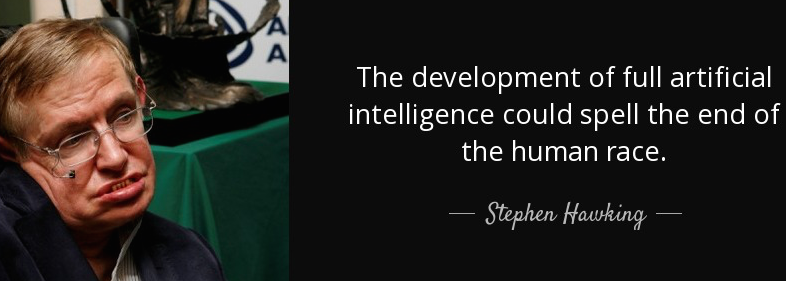
\includegraphics[height=0.19\textwidth]{figs/SH.png} \hspace{.2cm}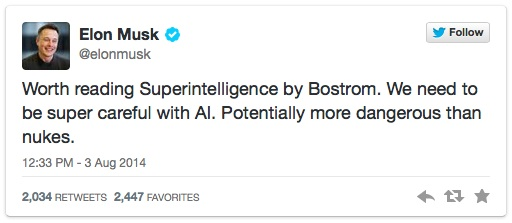
\includegraphics[height=0.19\textwidth]{figs/EM}
    \pause

      \vspace{0.2cm}
        {\hspace{0cm}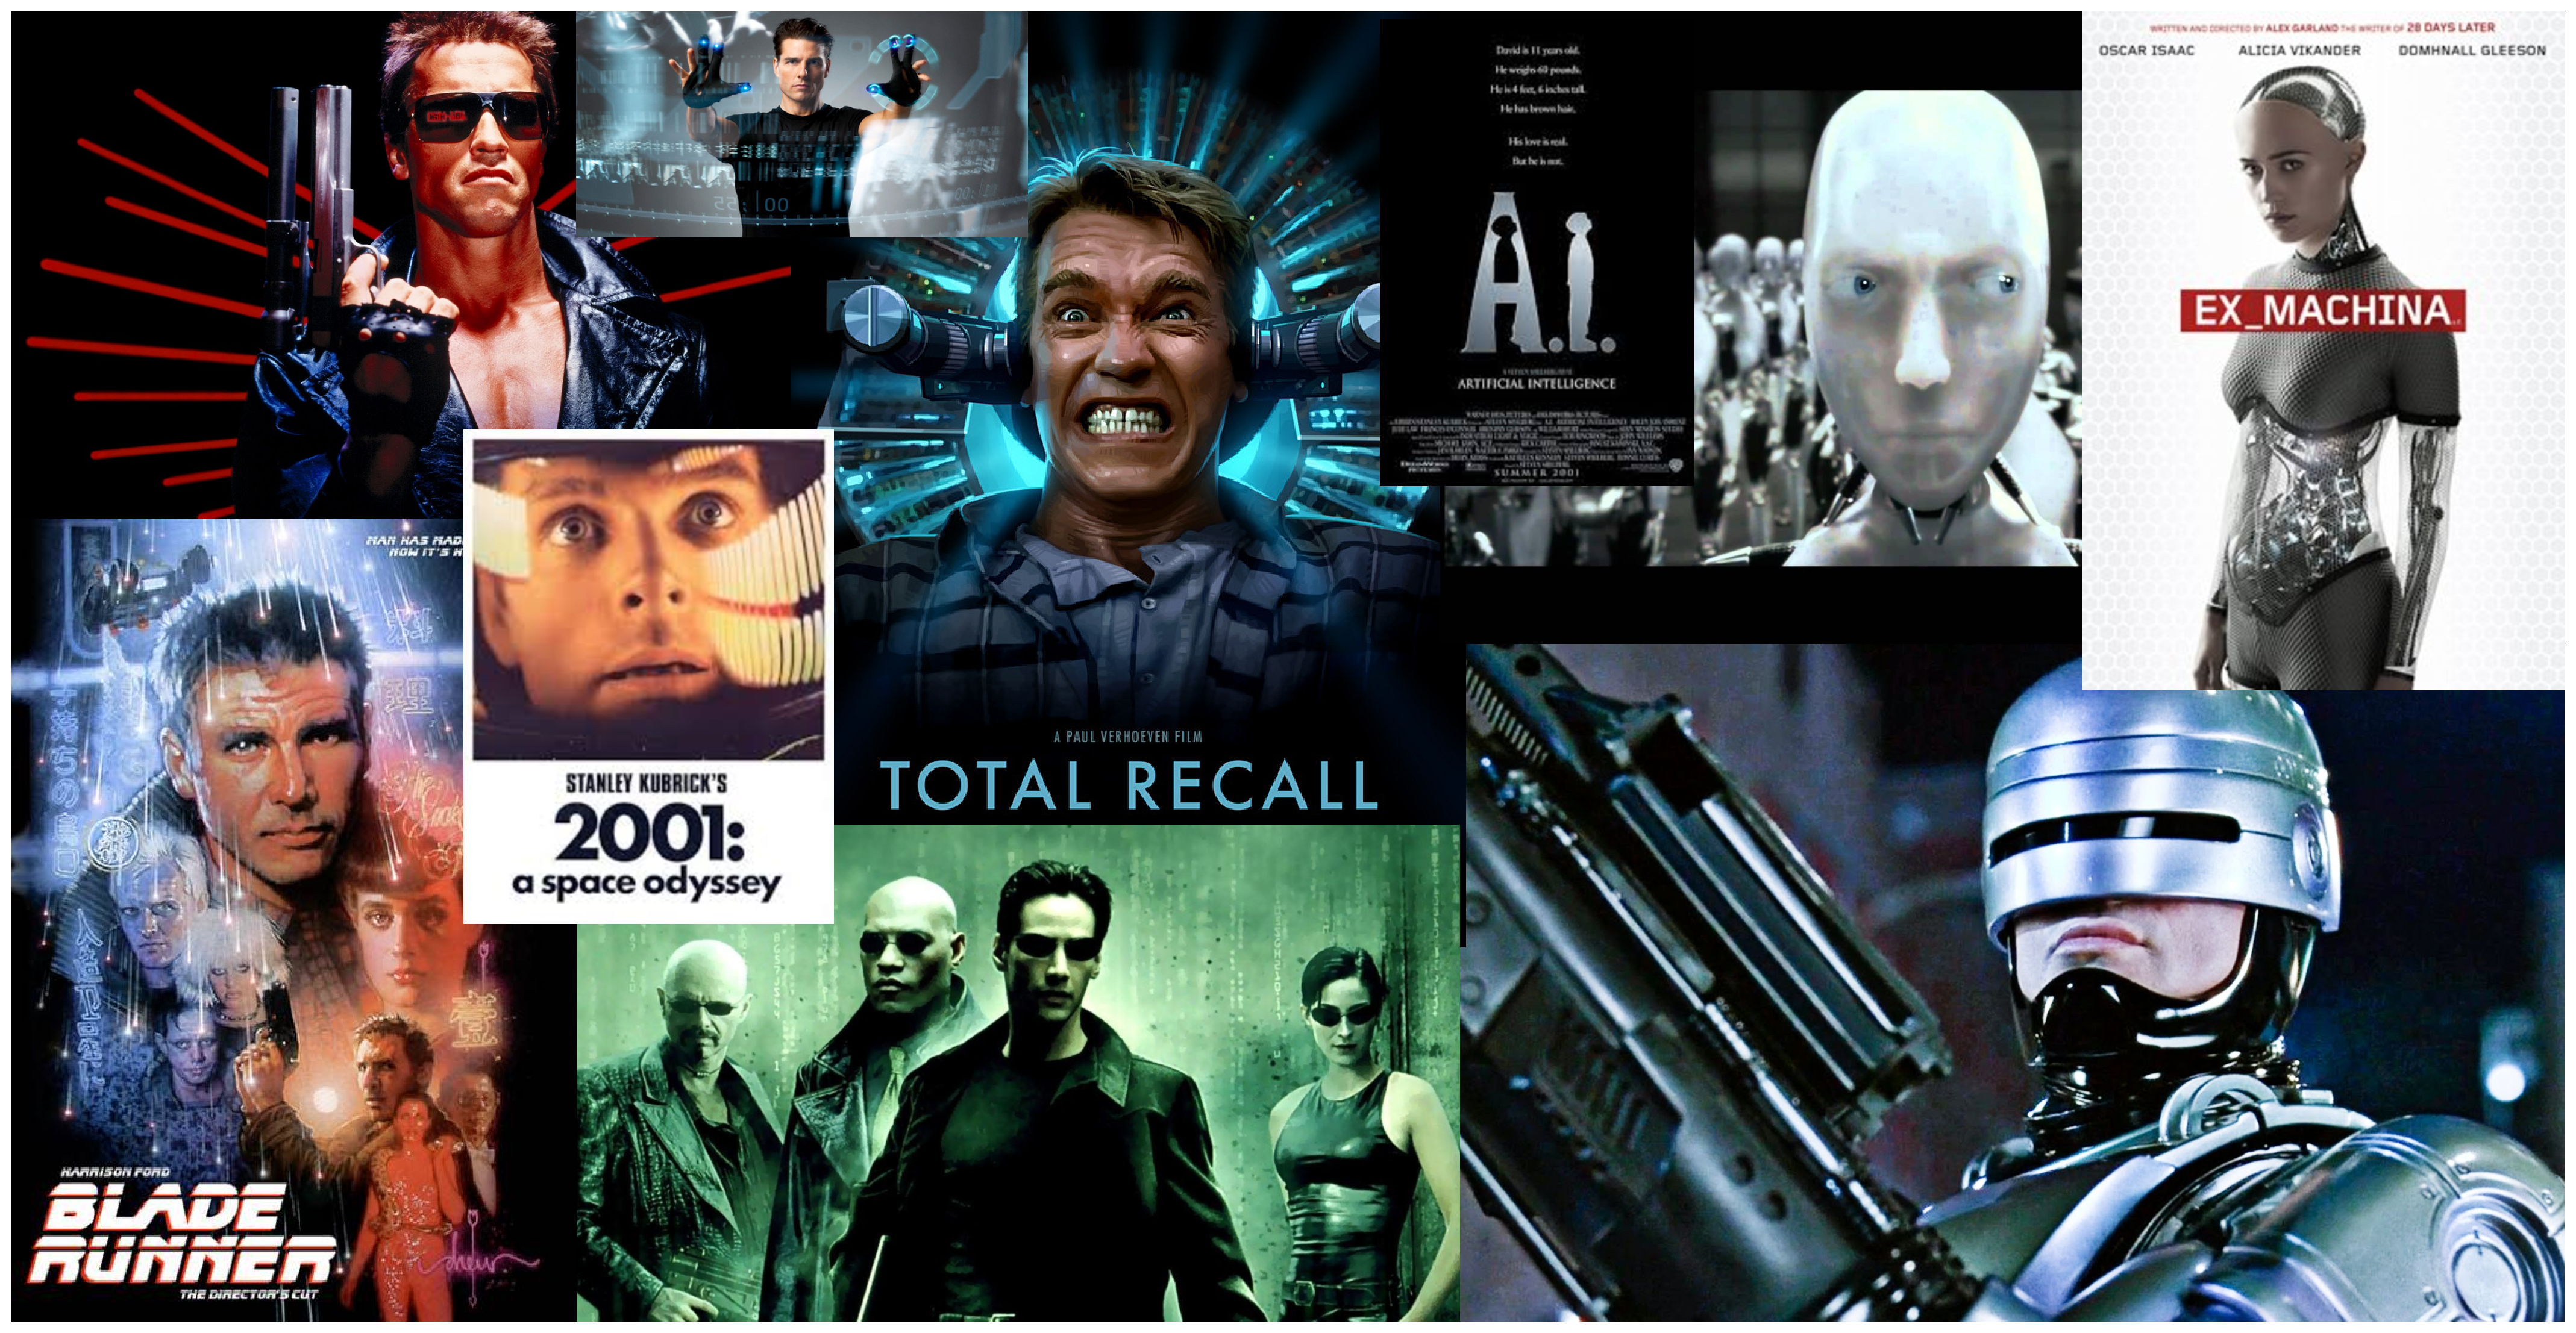
\includegraphics[width=0.99\textwidth]{figs/movies}}



}





  \section{Section no.1}
  \frame[t]{\frametitle{Bases de la Inteligencia Artificial\footfullcite{russel_norvig_2003}: 1) Filosofía: }
  (384-322 A.C.) Aristóteles: Análisis formal de los silogismos\\
  (1232–1315) Ramon Llull: Máquinas para razonar\\
  (1588-1679) Thomas Hobbes: razonamiento a través de cálculos numéricos - \textit{Leviathan}\\

  \begin{textblock}{1}(1,7)
    
\includegraphics[width=5\textwidth]{figs/silogismo}
  \end{textblock}

  \begin{textblock}{1}(7,7)
    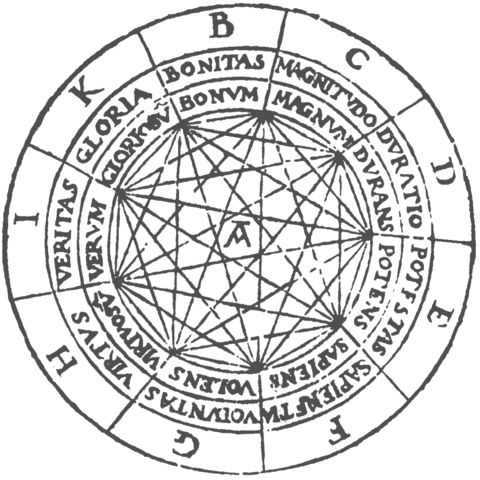
\includegraphics[width=3\textwidth]{figs/llull}
  \end{textblock}

  \begin{textblock}{1}(11,7)
    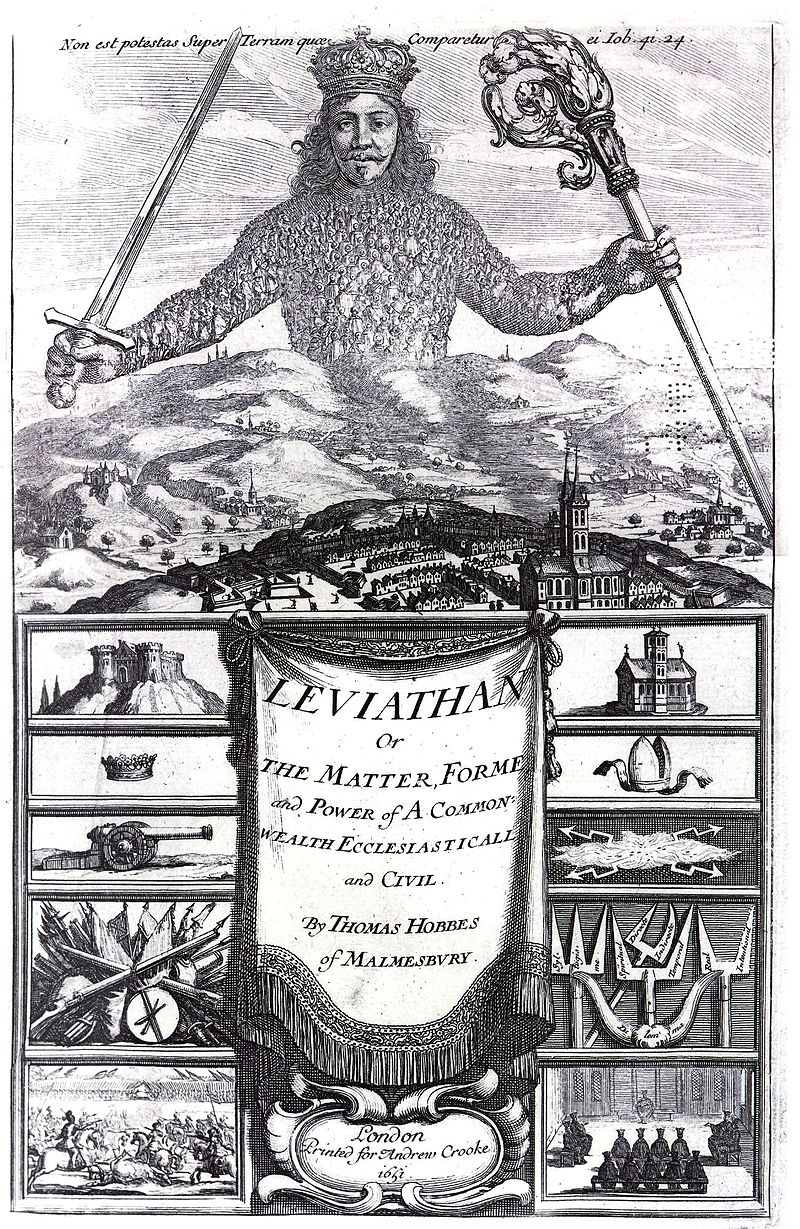
\includegraphics[width=3\textwidth]{figs/Leviathan}
  \end{textblock}

  }

  \frame[t]{\frametitle{Bases de la Inteligencia Artificial\footfullcite{russel_norvig_2003}: 1.5) Filosofía: }
  (1623-1662) Blaise Pascal: La pascaline, primera calculadora mecánica:
  \centerline{\textit{Los efectos de esta máquina son más}}
  \centerline{\textit{cercano a la inteligencia que cualquier acto animal}}
  (1596-1650) Rene Descartes: mente y materia implica carencia de libre albedrío. \\
  \qquad \qquad $\Rightarrow$ Racionalismo y dualismo $\neq$ materialismo\\
  Fuente del conocimiento: Empiricismo, racionalismo y sceptisismo (Bacon, Locke, Hume, Wittgenstein, Russell)

  \begin{textblock}{1}(1,10)
    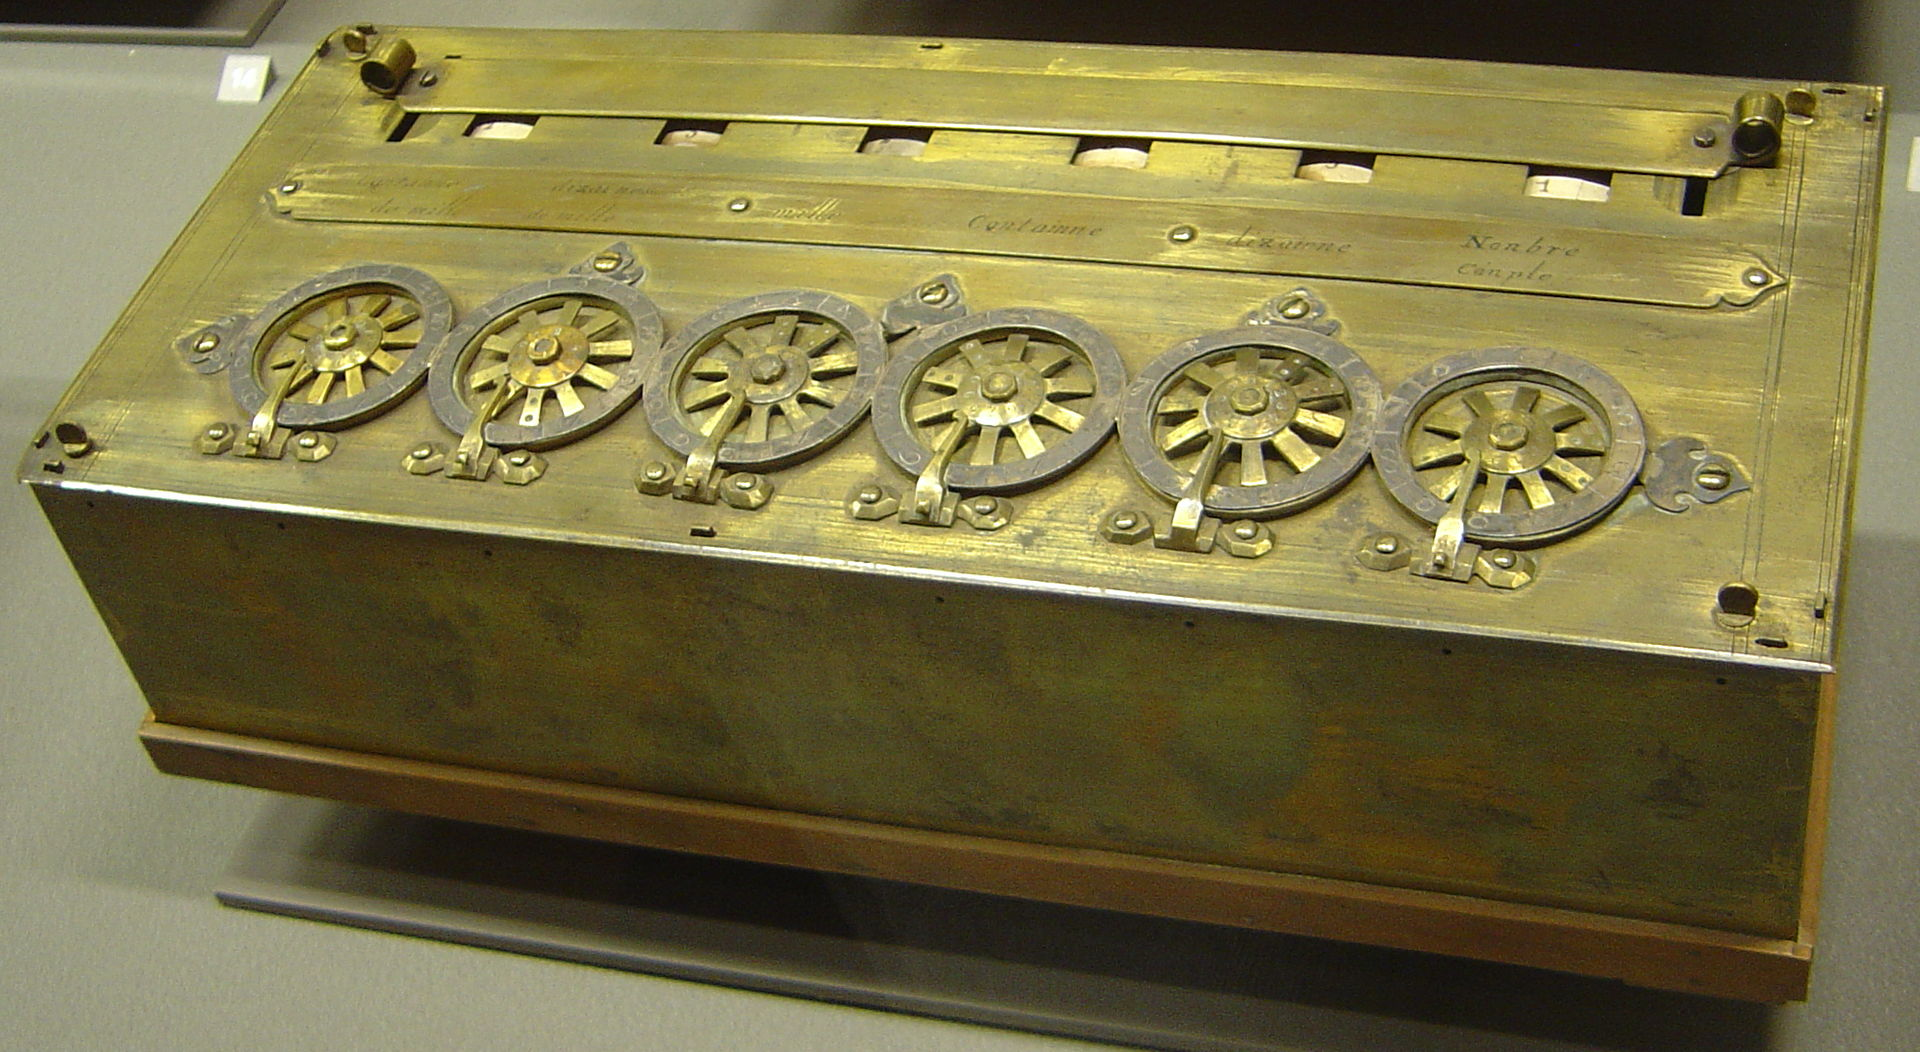
\includegraphics[width=4\textwidth]{figs/pascaline}
  \end{textblock}

  \begin{textblock}{1}(7,10)
    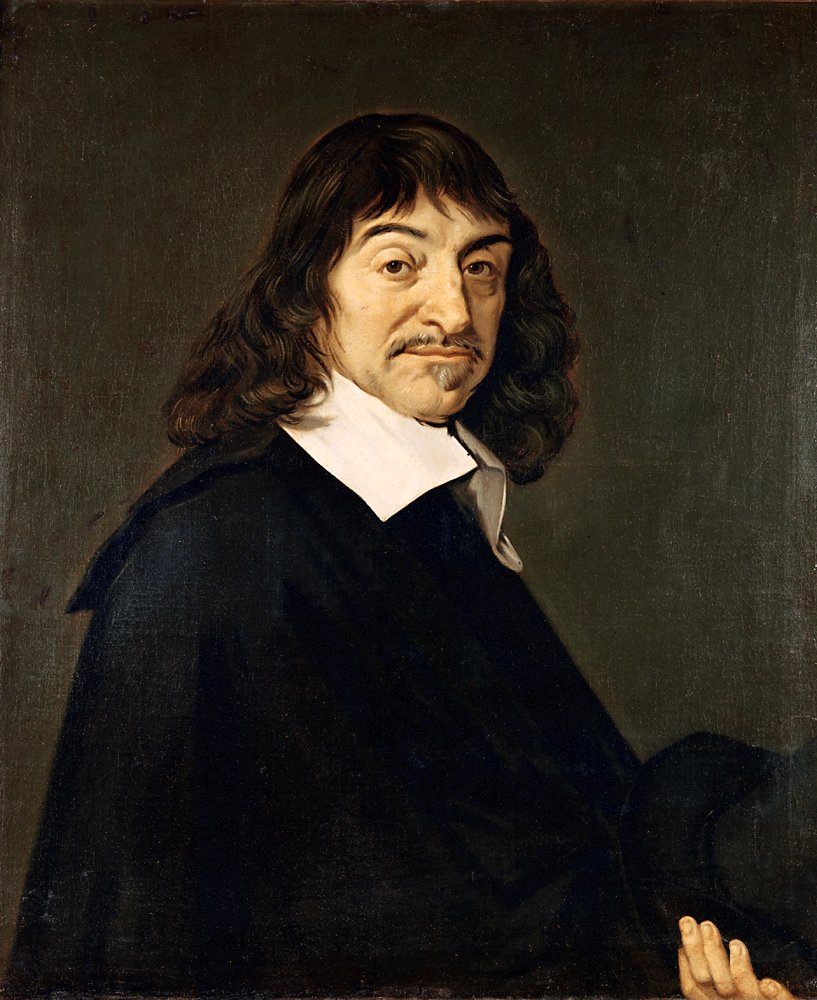
\includegraphics[width=2\textwidth]{figs/descartes}
  \end{textblock}

  \begin{textblock}{1}(11,9)
    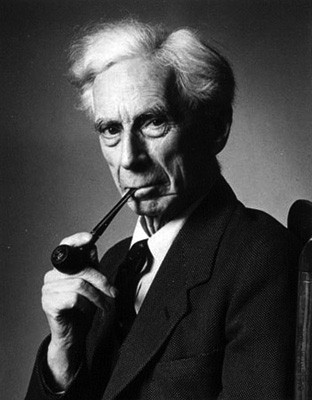
\includegraphics[width=2\textwidth]{figs/russell}
  \end{textblock}

  \begin{textblock}{1}(12,11.5)
    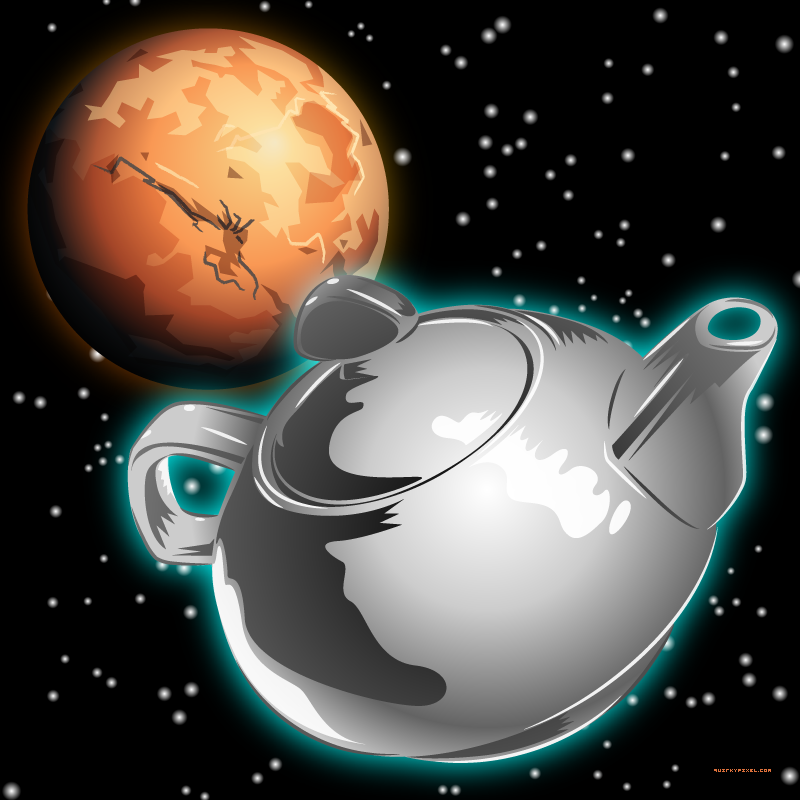
\includegraphics[width=2\textwidth]{figs/teapot}
  \end{textblock}
  } 


    \frame[t]{\frametitle{Bases de la Inteligencia Artificial\footfullcite{russel_norvig_2003}: 2) Matemáticas: }
    Boole (1847) y Frege (1879): Lógica Booleana y proposicional\\
    Russell and Whitehead (1913): \textit{Principia Matematica}\\
    (1930-1931) G\"odel: Teoremas de completitud e incompletitud --- los límites existen\\
    (1936) Turing-Church: La máquina de Turing puede computar cualquier función computable
    \begin{textblock}{1}(1,8)
      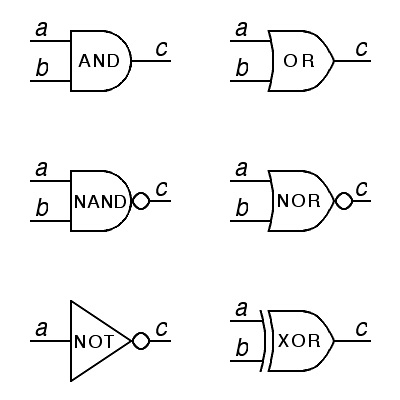
\includegraphics[width=3\textwidth]{figs/logic}
    \end{textblock}

    \begin{textblock}{1}(5,7.5)
      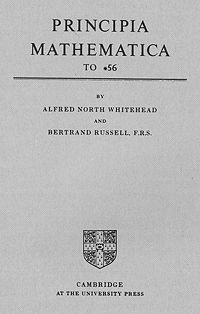
\includegraphics[width=2.5\textwidth]{figs/principia1}
    \end{textblock}

    \begin{textblock}{1}(7,10)
      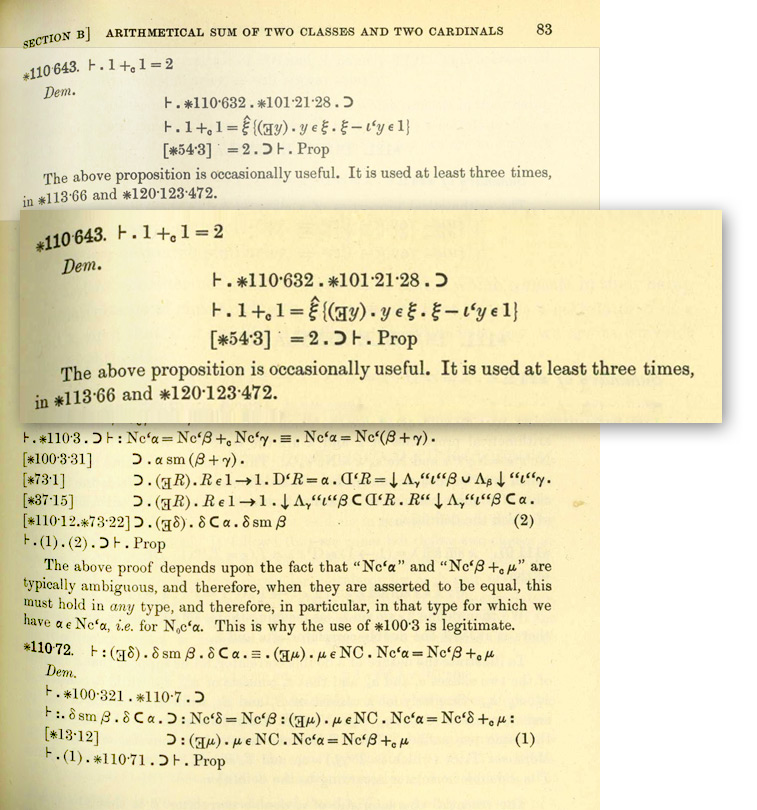
\includegraphics[width=3\textwidth]{figs/principia2}
    \end{textblock}

    \begin{textblock}{1}(11,8)
      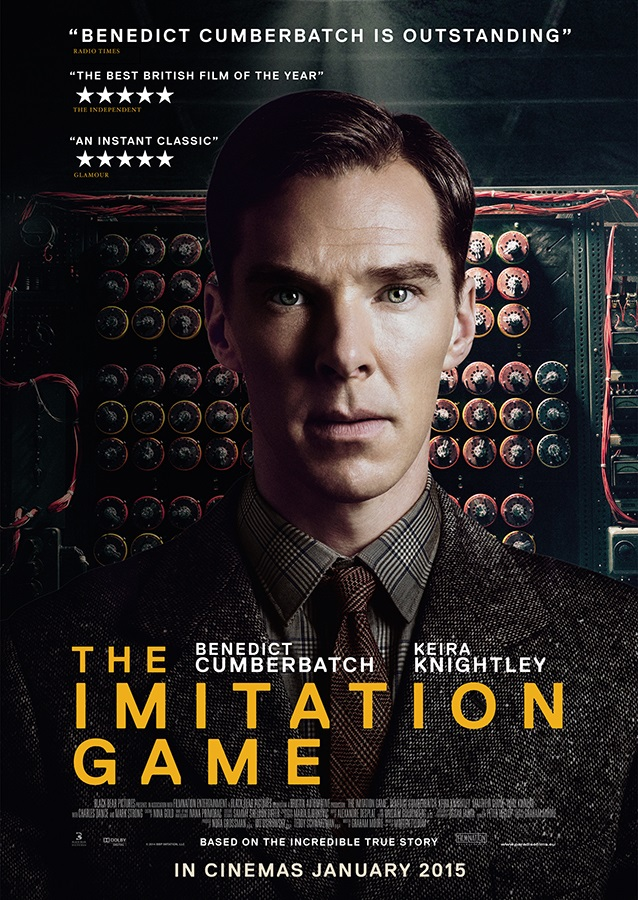
\includegraphics[width=3\textwidth]{figs/turing}
    \end{textblock}

    }

      \frame[t]{\frametitle{Bases de la Inteligencia Artificial: 3) Probabilidades: }

      Ley de evidencia: Cardamo, Pascal, Fermat (1500-1600)\\
      Matemáticas formales: Bernoulli (1700)\\
      Combinación con datos: Laplace y Gauss (1800)\\
      Estadística: Fisher (1900)\\
      Teoría de Medida: Kolmogorov (1933)

      Distintas interpretaciones de probabilidad\footfullcite{casella_2008}:

      \begin{textblock}{1}(5,7)
        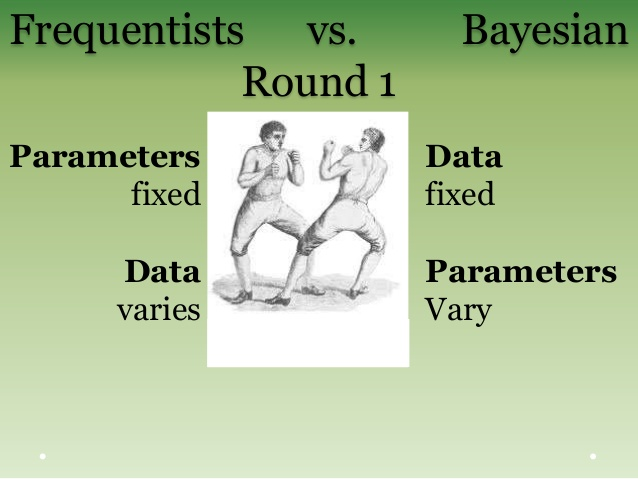
\includegraphics[width=6\textwidth]{figs/FvsB}
      \end{textblock}
\vspace{4cm}
\footnotesize{ \red{Lectura próxima clase:} \href{http://www.nytimes.com/2014/09/30/science/the-odds-continually-updated.html}{Frecuentistas versus Bayesiano} y \href{http://simplystatistics.org/2014/10/13/as-an-applied-statistician-i-find-the-frequentists-versus-bayesians-debate-completely-inconsequential/ }{respuesta de un estadístico}}



      }










      %%%%%%%%

      \frame[t]{\frametitle{Artificial Intelligence}
      \small
      \vspace{1em}
      $\red{\bullet}$ Intelligence is crucial for us: unlike the rest of the animal kingdom, we do not need to evolve to adapt\\
      \pause
      $\red{\bullet}$ We have always been interested in understand intelligence but AI goes even further: it aims to replicate it.\\
      \pause
      \vspace{2em}
      \centerline{{---Definitions of AI\footfullcite{russel_norvig_2003}---}}
  \begin{table}[]
      \scriptsize
  \centering
  \begin{tabular}{|l|c|c|}
  \hline
                                     & \textbf{Human}                                                                                                                                                                                   & \textbf{Rational}                                                                                                                          \\ \hline
  \textbf{Think}                     & \begin{tabular}[c]{@{}c@{}}``{[}automation of{]} activities associated \\ with human thinking, activities such \\ as descision-making, problem solving,\\  learning" (Bellman, 1978)\end{tabular} & \begin{tabular}[c]{@{}c@{}}``Study of mental faculties \\ through the use of computational \\ models" (Charniak et al., 1985)\end{tabular} \\ \hline
  \multicolumn{1}{|c|}{\textbf{Act}} & \begin{tabular}[c]{@{}c@{}}``The art of creating machines that \\ perform functions that require \\ intelligence when performed \\ by people" (Kurzweil, 1990)\end{tabular}                       & \begin{tabular}[c]{@{}c@{}}``Study and design of intelligent \\ agents" (Poole et al., 1998)\end{tabular}                                   \\ \hline
  \end{tabular}
  \end{table}


    }
        %%%%%%%%%%

           \begin{frame}[plain]
        \frametitle{Artificial Intelligence}
        \small
        \vspace{1em}
        $\red{\bullet}$ Intelligence is crucial for us: unlike the rest of the animal kingdom, we do not need to evolve to adapt\\
        $\red{\bullet}$ We have always been interested in understand intelligence but AI goes even further: it aims to replicate it.\\
        \vspace{2em}
        \centerline{{---Definitions of AI\footfullcite{russel_norvig_2003}---}}
        % Please add the following required packages to your document preamble:
      % \usepackage[table,xcdraw]{xcolor}
      % If you use beamer only pass "xcolor=table" option, i.e. \documentclass[xcolor=table]{beamer}
      \begin{table}[]
        \scriptsize
      \centering
      \begin{tabular}{|l|c|c|}
      \hline
                                         & \textbf{Human}                                                                                                                                                                                                            & \textbf{Rational}                                                                                                                           \\ \hline
      \textbf{Think}                     & \cellcolor[HTML]{FFFFFF}\begin{tabular}[c]{@{}c@{}}``{[}automation of{]} activities associated \\ with human thinking, activities such \\ as descision-making, problem solving,\\  learning" (Bellman, 1978)\end{tabular} & \begin{tabular}[c]{@{}c@{}}``Study of mental faculties \\ through the use of computational \\ models" (Charniak et al., 1985)\end{tabular} \\ \hline
      \multicolumn{1}{|c|}{\textbf{Act}} & \cellcolor[HTML]{FD6864}\begin{tabular}[c]{@{}c@{}}``The art of creating machines that \\ perform functions that require \\ intelligence when performed \\ by people" (Kurzweil, 1990)\end{tabular}                       & \begin{tabular}[c]{@{}c@{}}``Study and design of intelligent \\ agents" (Poole et al., 1998)\end{tabular}                                    \\ \hline
      \end{tabular}
      \end{table}


      \end{frame}






\frame[t]{
\begin{textblock}{1}(1.5,0)
  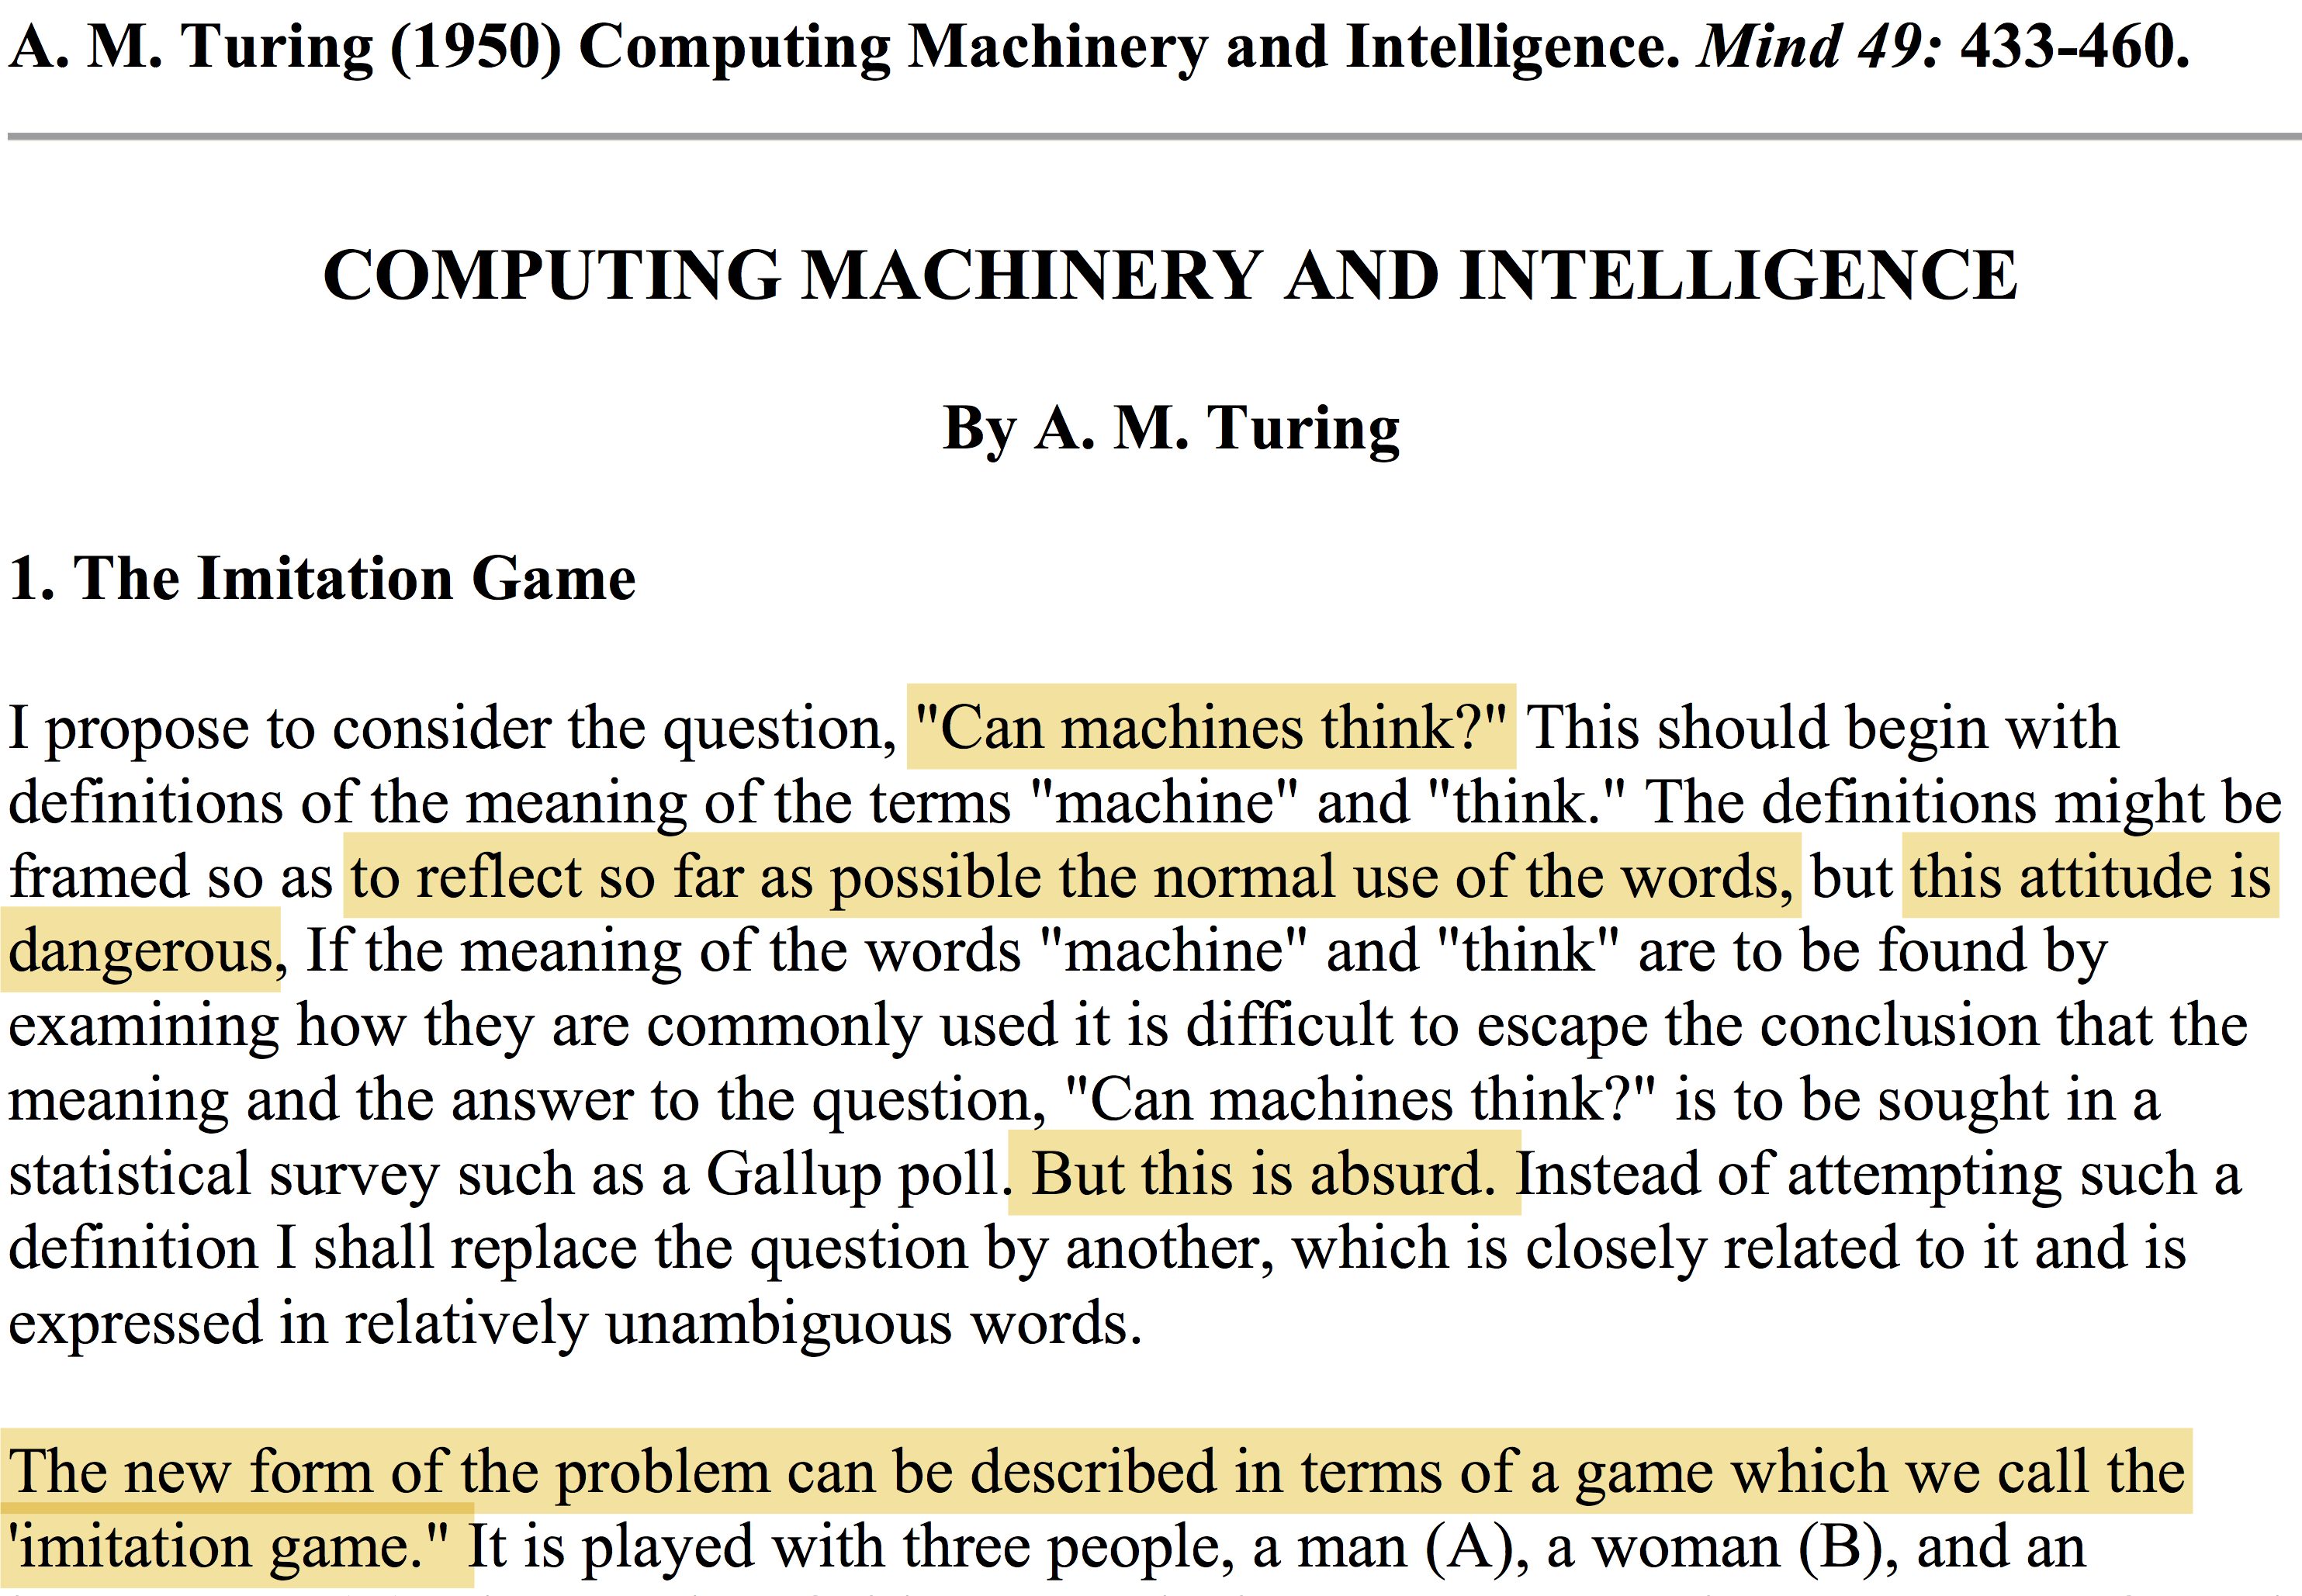
\includegraphics[width=13\textwidth]{figs/AT}
\end{textblock}

\begin{textblock}{1}(13.3,2)
  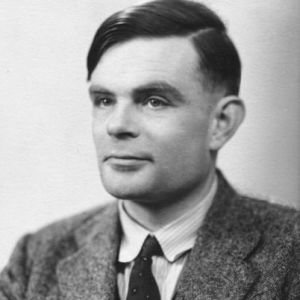
\includegraphics[width=2\textwidth]{figs/ATp}
\end{textblock}

\begin{textblock}{1}(4.5,12)
  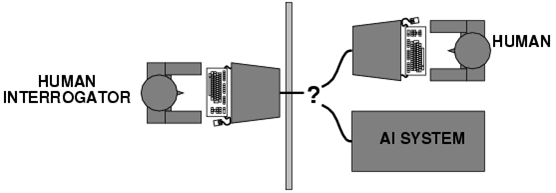
\includegraphics[width=7\textwidth]{figs/turing-test}
\end{textblock}

}




\frame[t]{\frametitle{Requerimientos para aprobar el test de Turing\footfullcite{russel_norvig_2003}}
\begin{itemize}
  \item \blue{Procesamiento de lenguaje natural:} Habilidad de comunicarse
  \item \blue{Representación de información:} Almacenamiento de \textit{conocimiento}
  \item \blue{Razonamiento:} usar información para concluir
  \item \red{Aprendizaje de máquinas:} construir conocimiento y adaptarse
  \item \blue{Visón computacional$^*$:} percibir el entorno
  \item \blue{Robótica$^*$:} Interacturar con el entorno
\end{itemize}

\redm{$\star$ AM ha dejado de ser una componente exclusiva de IA y se ha convertido en un fin en sí mismo con aplicaciones en variadas disciplinas.}

}





  \frame{\frametitle{Aprendizaje de Máquinas entre nosotros}
  \begin{textblock}{1}(1,2)
    
\includegraphics[width=6\textwidth]{figs/trueskill}
  \end{textblock}

  \begin{textblock}{1}(8,2)
    
\includegraphics[width=3\textwidth]{figs/skype}
  \end{textblock}

  \begin{textblock}{1}(11.5,1)
    
\includegraphics[width=4\textwidth]{figs/loan}
  \end{textblock}

  \begin{textblock}{1}(1,8)
    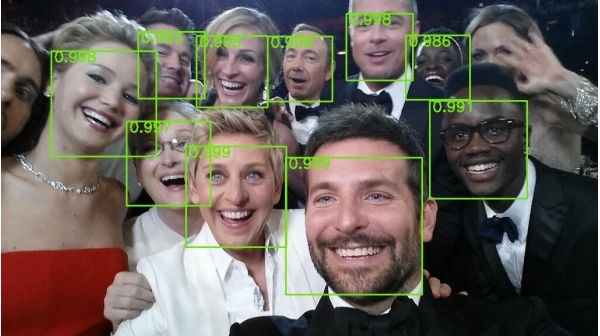
\includegraphics[width=6\textwidth]{figs/face_detection}
  \end{textblock}

  \begin{textblock}{1}(8,5)
    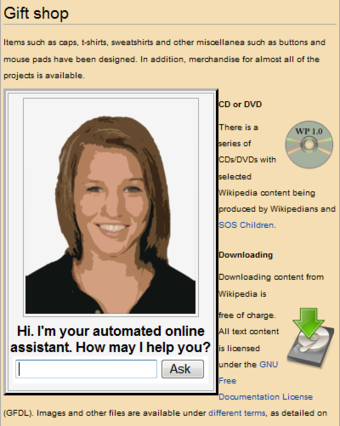
\includegraphics[width=3\textwidth]{figs/nlp}
  \end{textblock}

  \begin{textblock}{1}(13,9)
    
\includegraphics[width=2\textwidth]{figs/compression}
  \end{textblock}

  \begin{textblock}{1}(4.5,4.5)
    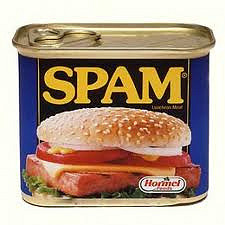
\includegraphics[width=2\textwidth]{figs/spam}
  \end{textblock}

  \begin{textblock}{1}(7.5,11)
    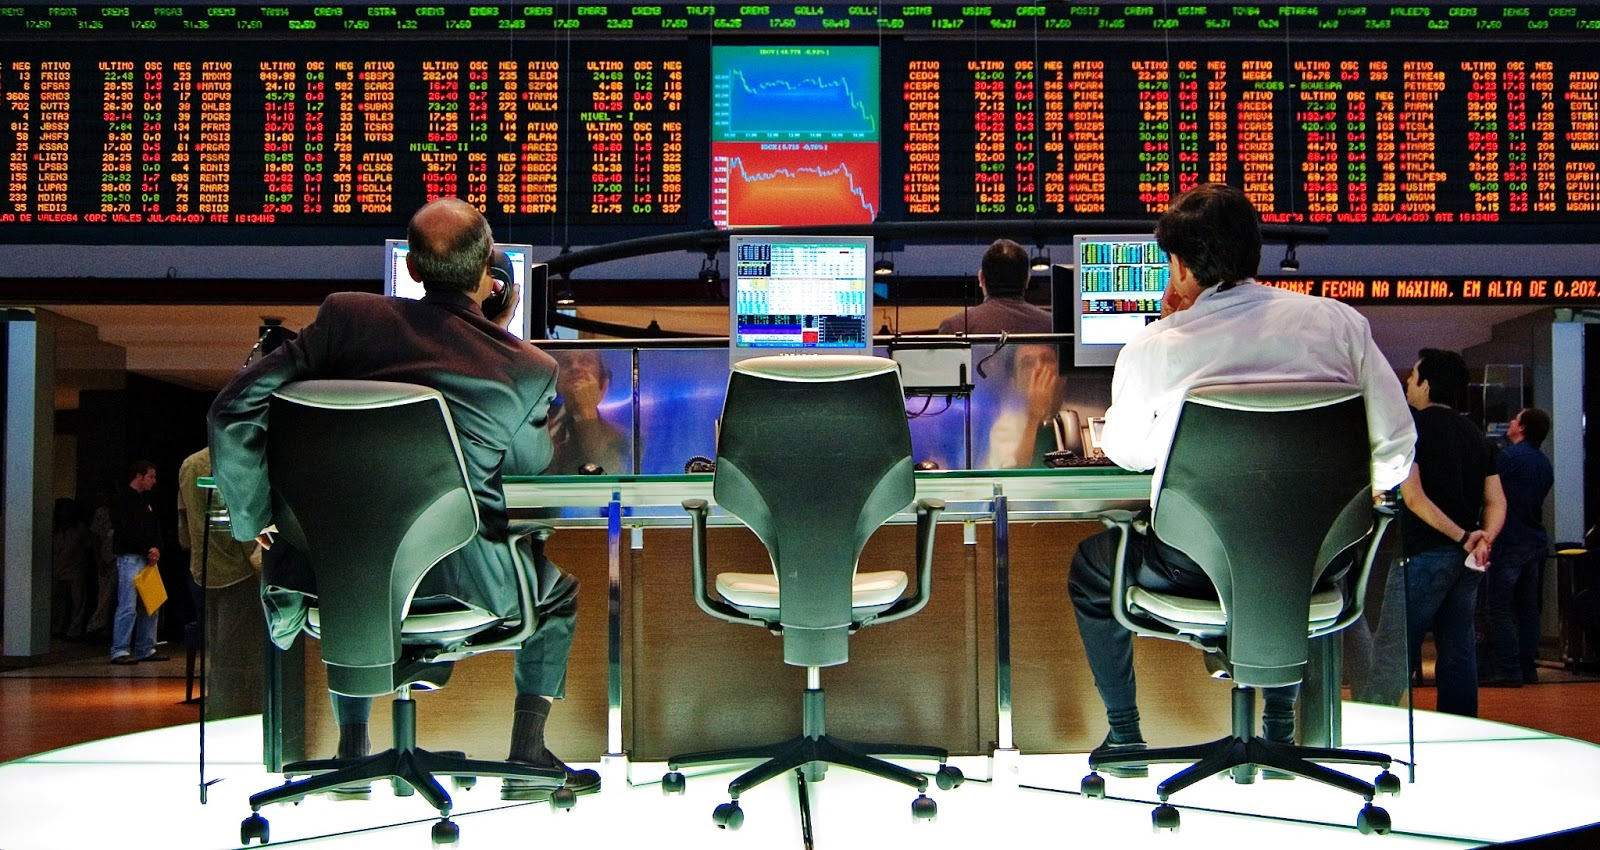
\includegraphics[width=6\textwidth]{figs/trading}
  \end{textblock}

  \begin{textblock}{1}(1.5,11)
    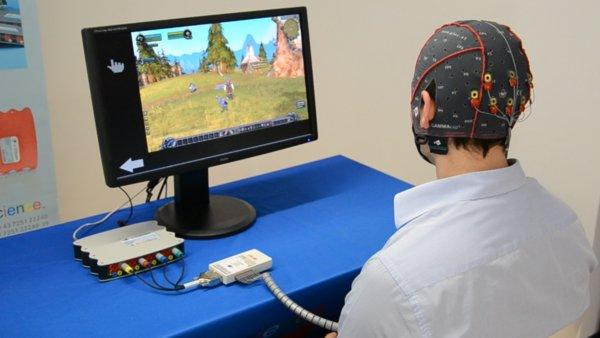
\includegraphics[width=6\textwidth]{figs/BCI}
  \end{textblock}


  }




    \frame{
    \begin{textblock}{1}(0.2,0.2)
      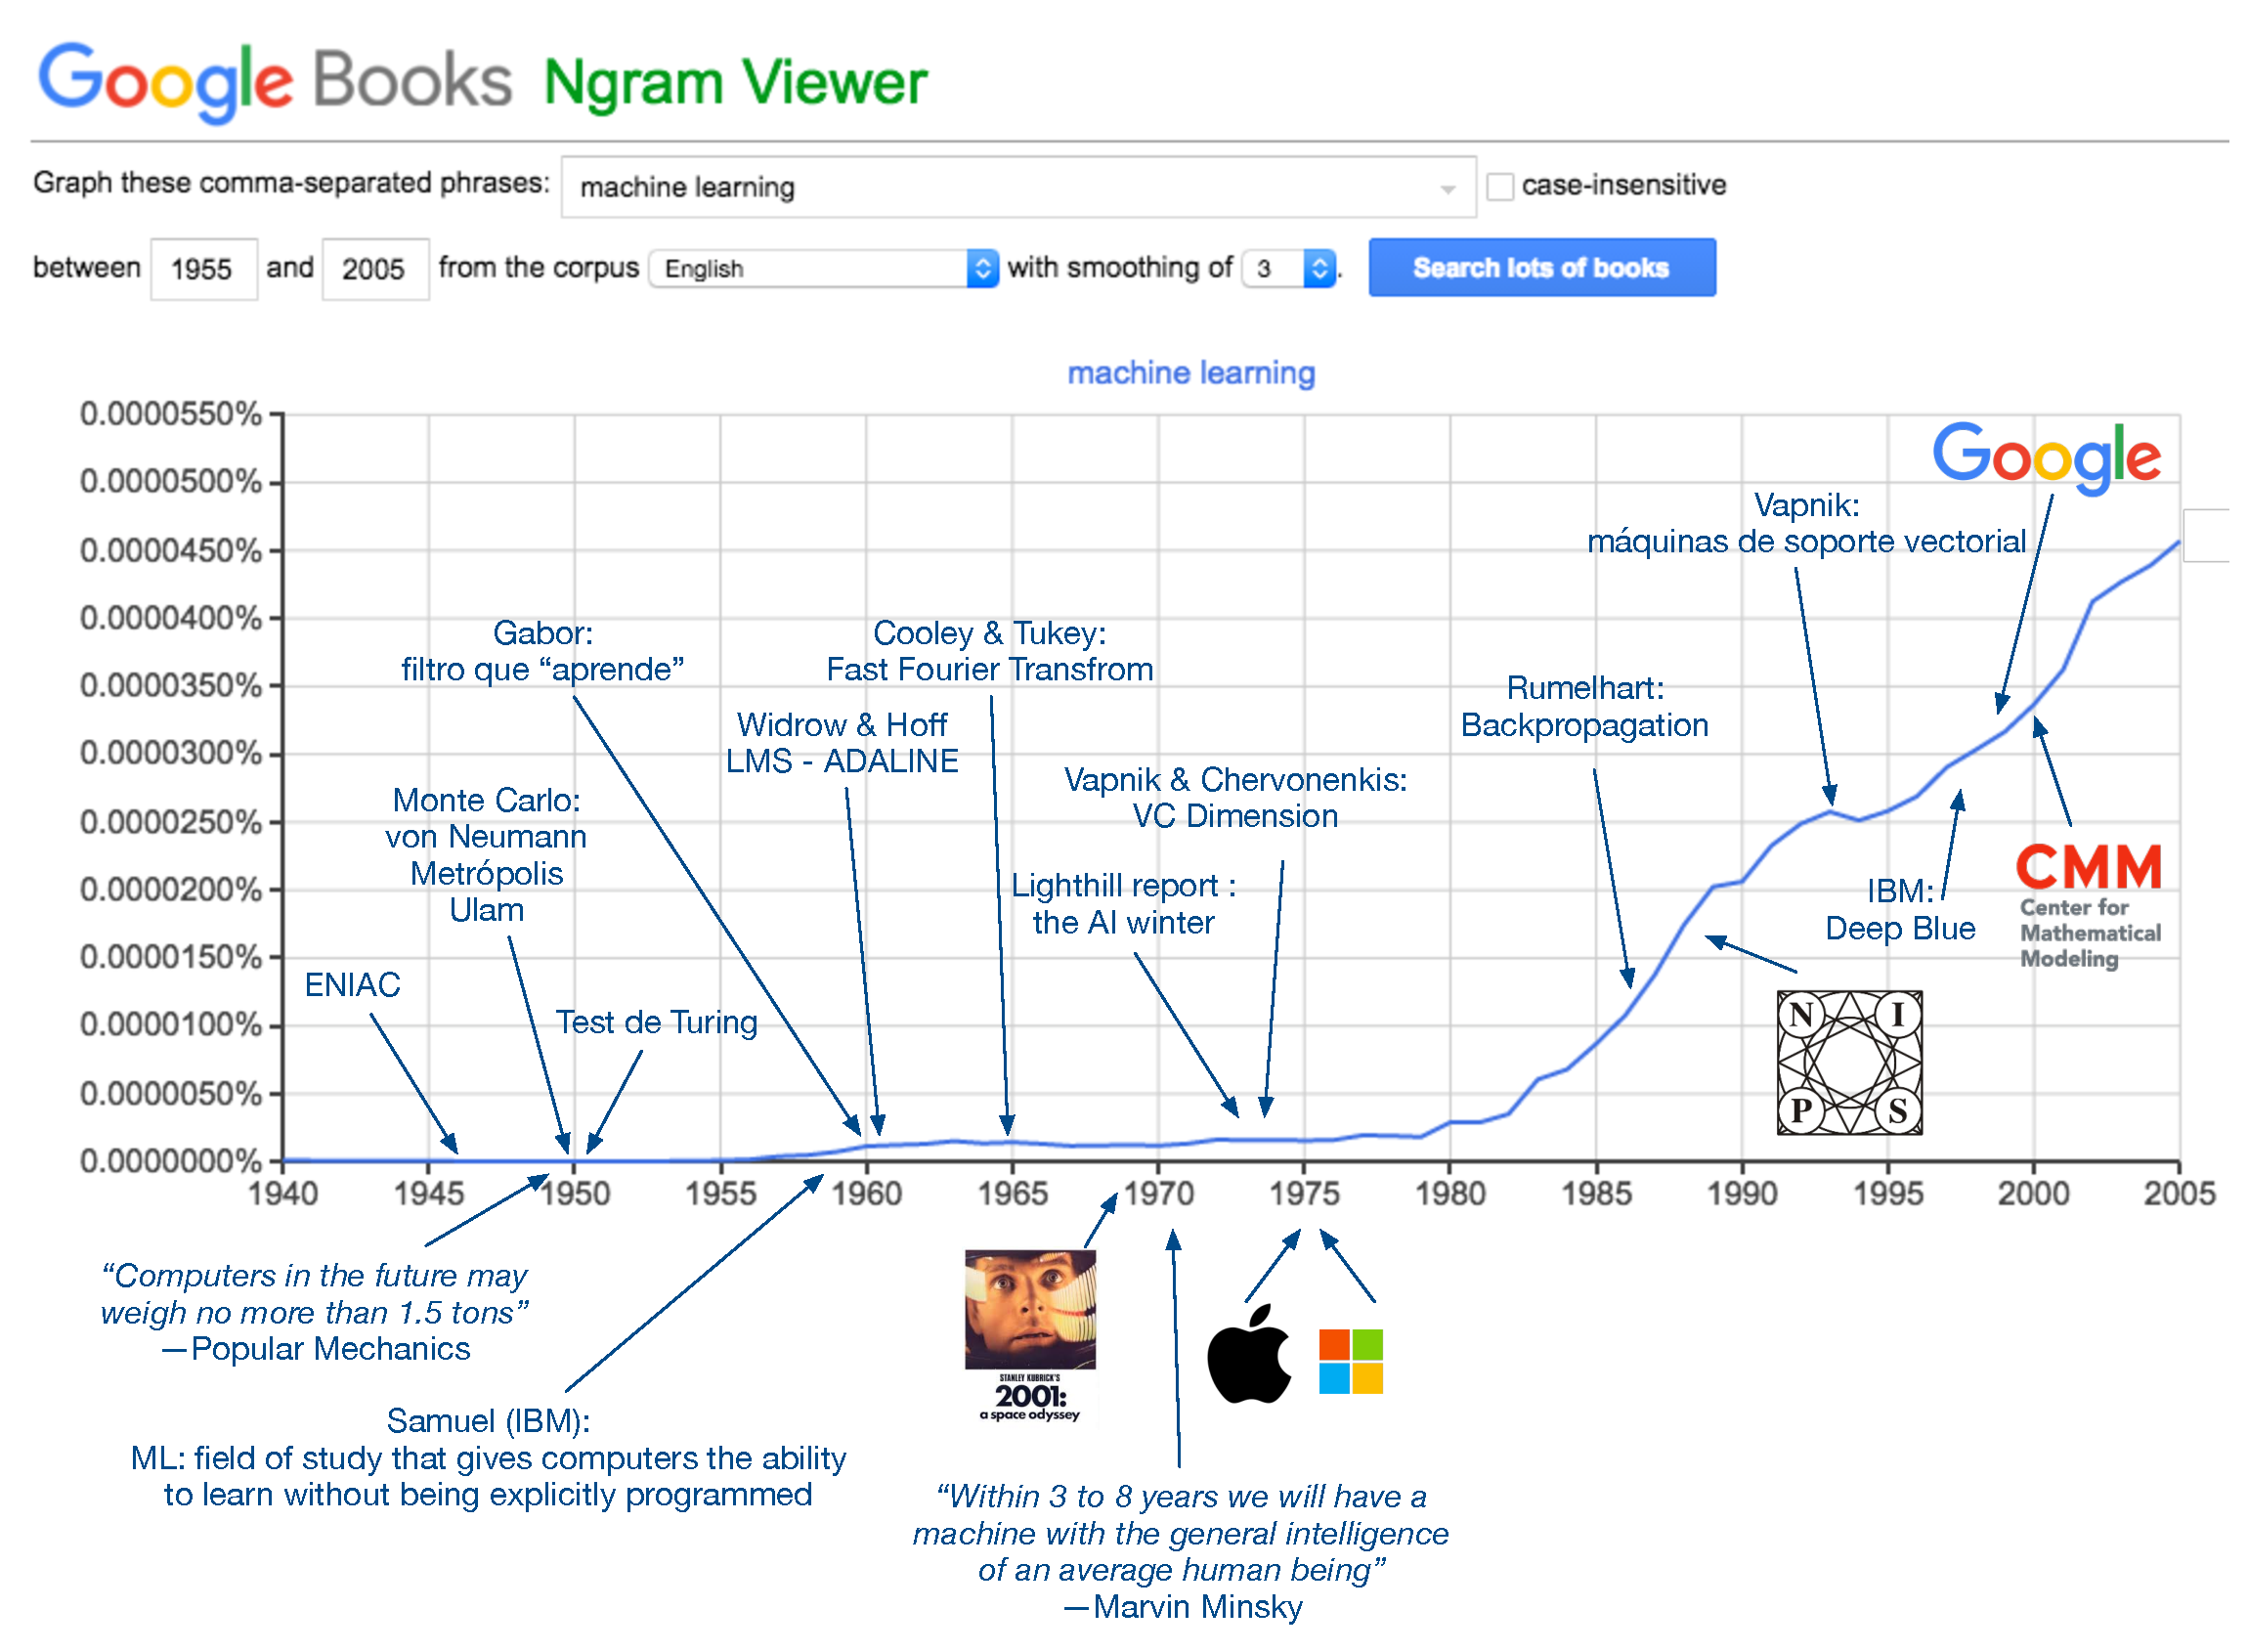
\includegraphics[width=15.5\textwidth]{figs/ngram}
    \end{textblock}


    }

    \frame{
    \begin{textblock}{1}(0.2,0.2)
      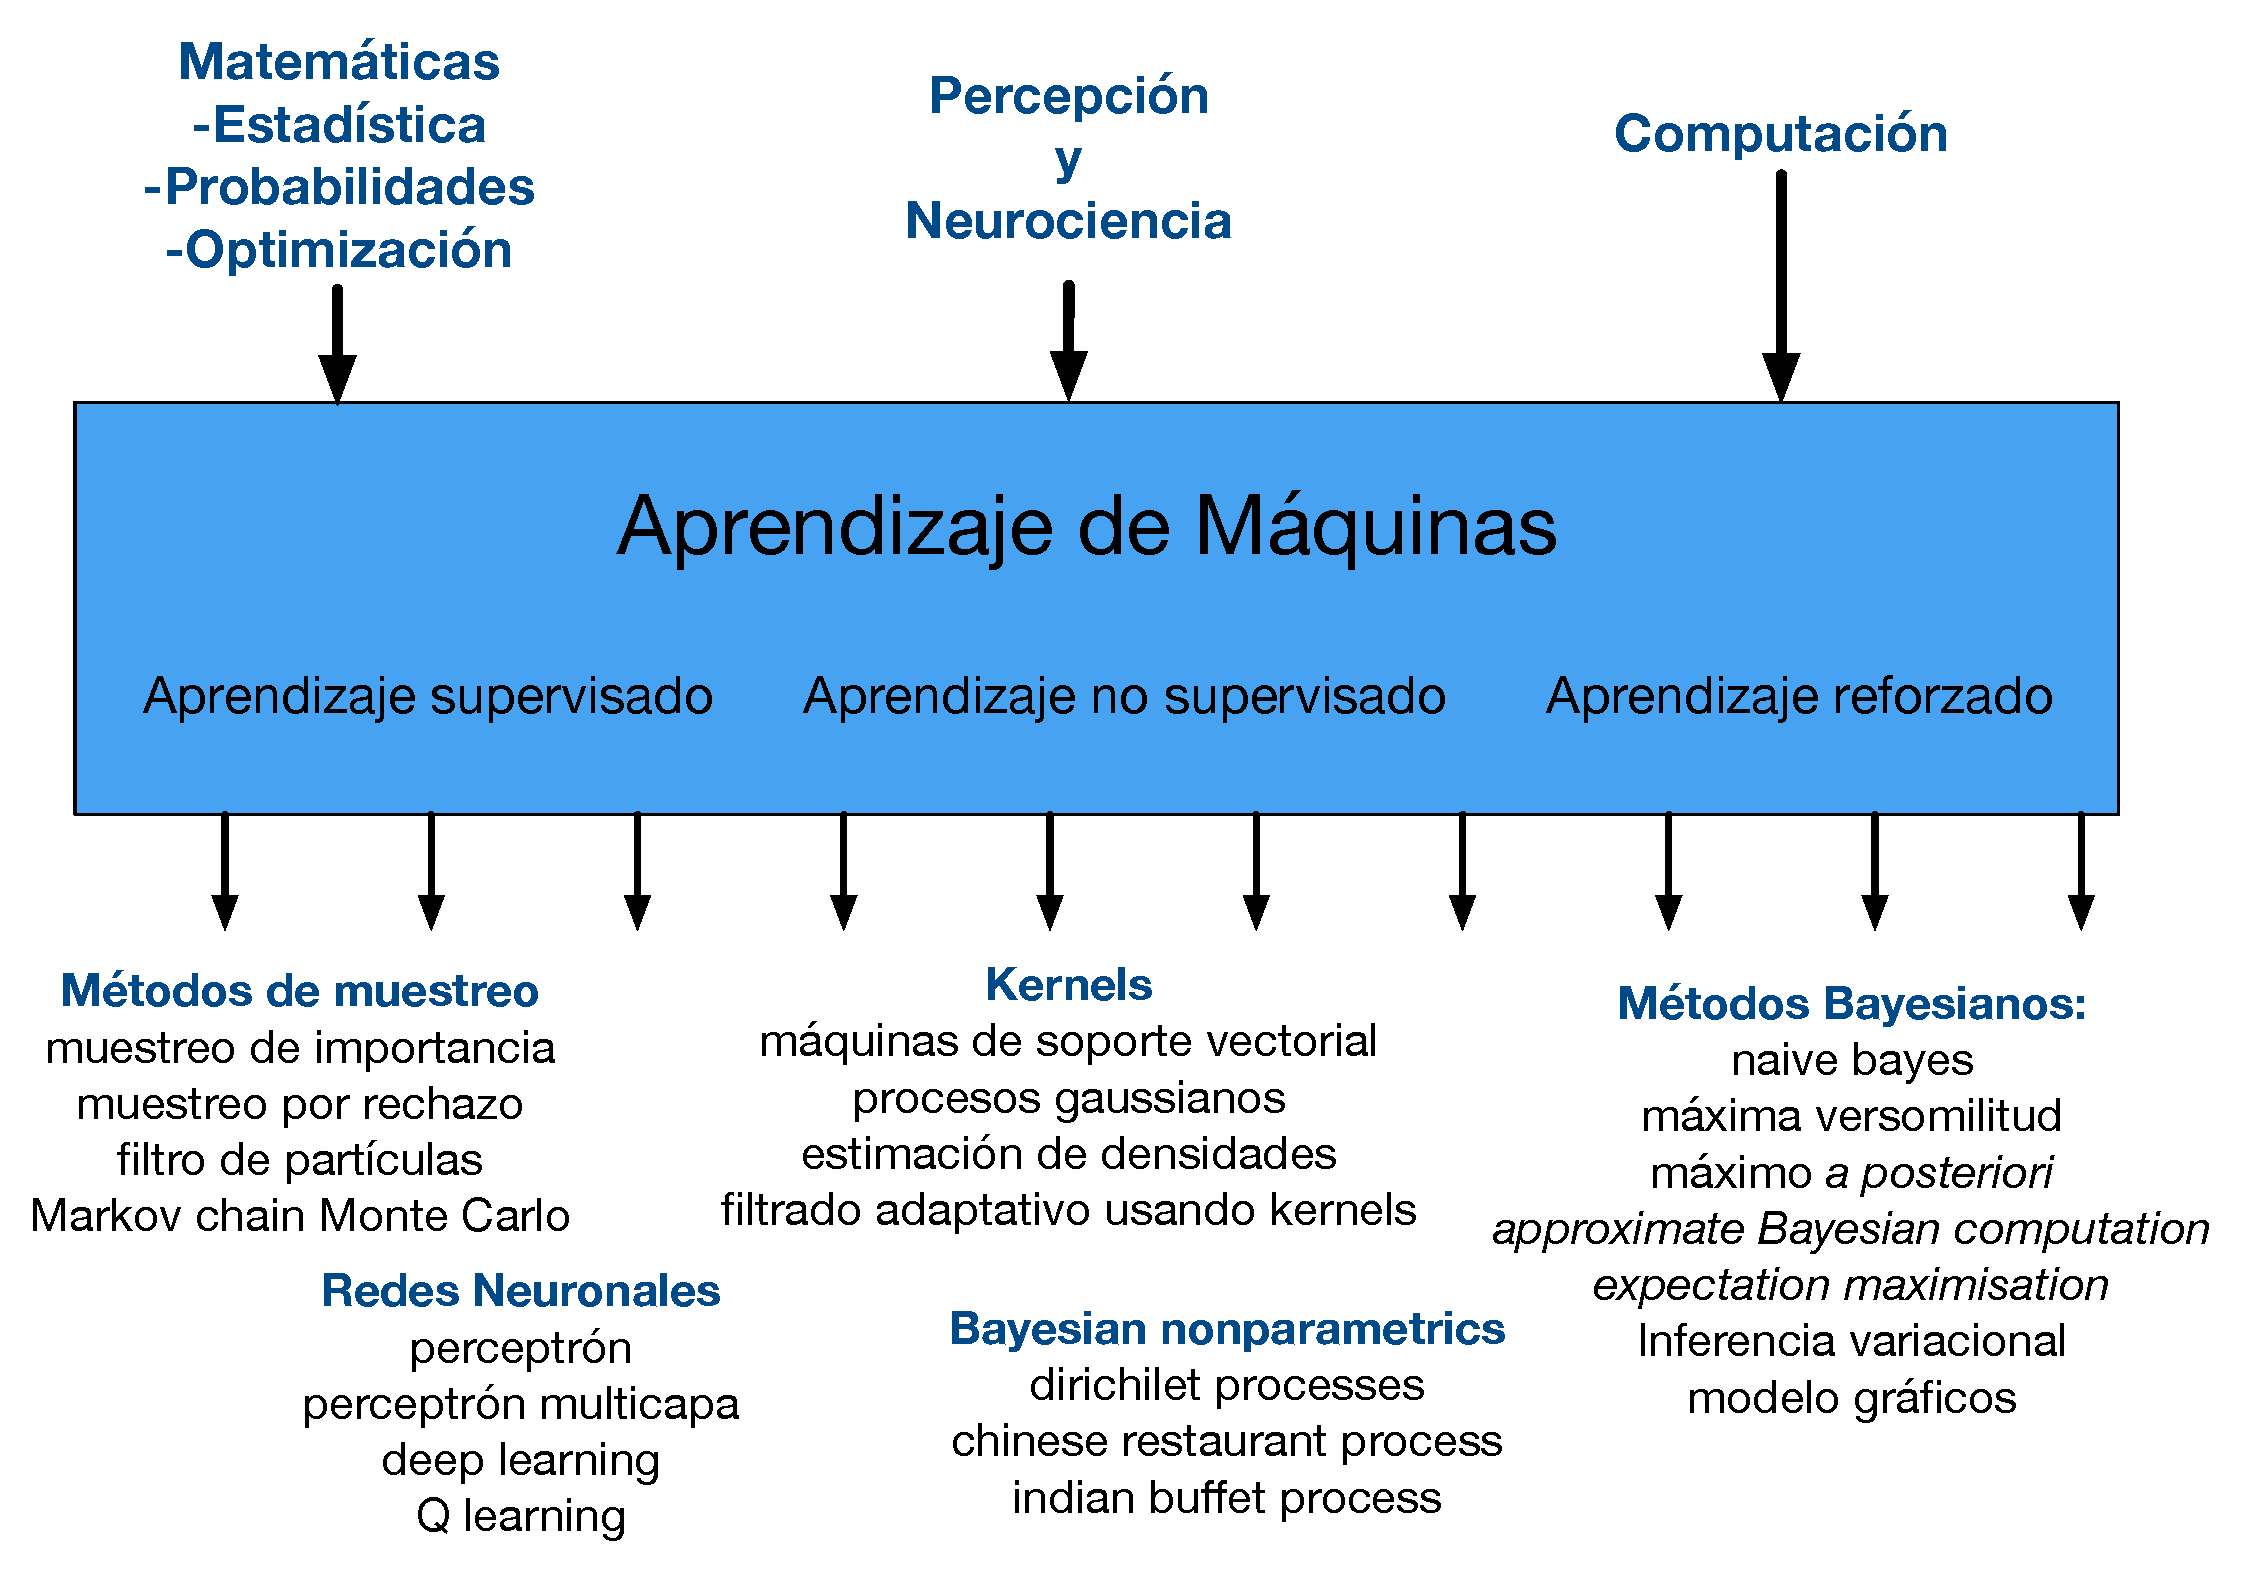
\includegraphics[width=15.5\textwidth]{figs/MLdiag}
    \end{textblock}


    }



  \frame[t]{\frametitle{Aprendizaje supervisado (Clasificación)\footfullcite{murphy_2012}}
  Encontrar el \text{mapeo} $x\rightarrow y$, en base a los datos $\{(x_i,y_i)\}_{i=1:N}$\\\vspace{0.3cm}
  \textbf{Ejemplo 1}\\
  -generalizar\\
  -decisiones\\
  \quad probabilísticas\\
\vspace{0.3cm}
  \textbf{Ejemplo 2}\\
  \begin{textblock}{1}(5,3)
    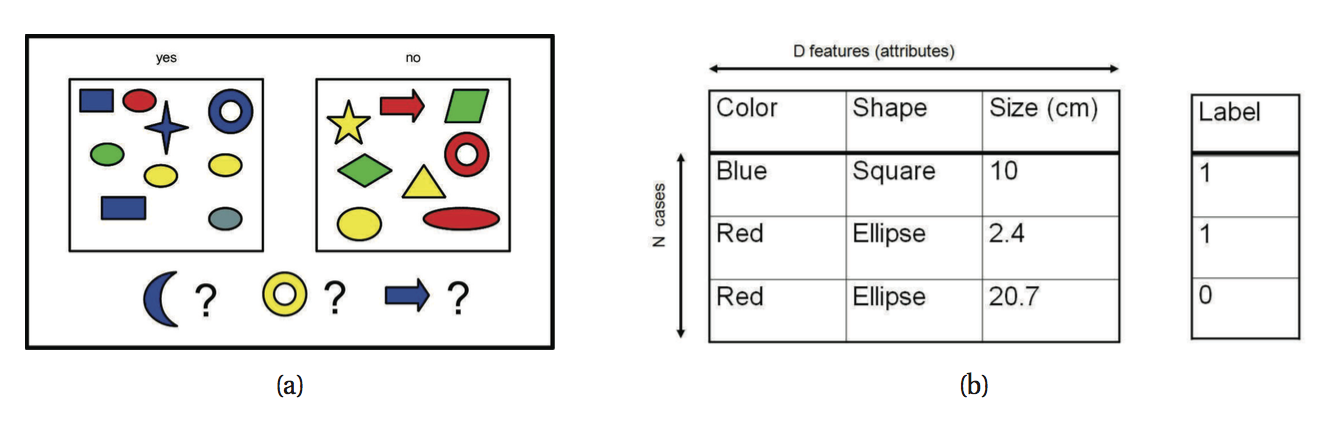
\includegraphics[width=10\textwidth]{figs/clasificacion}
  \end{textblock}
  \begin{textblock}{1}(1,8)
    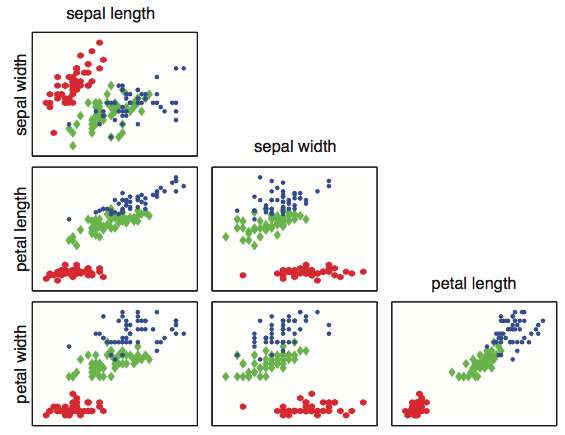
\includegraphics[width=6.5\textwidth]{figs/flores_features}
  \end{textblock}
    \begin{textblock}{1}(6.5,7.5)
    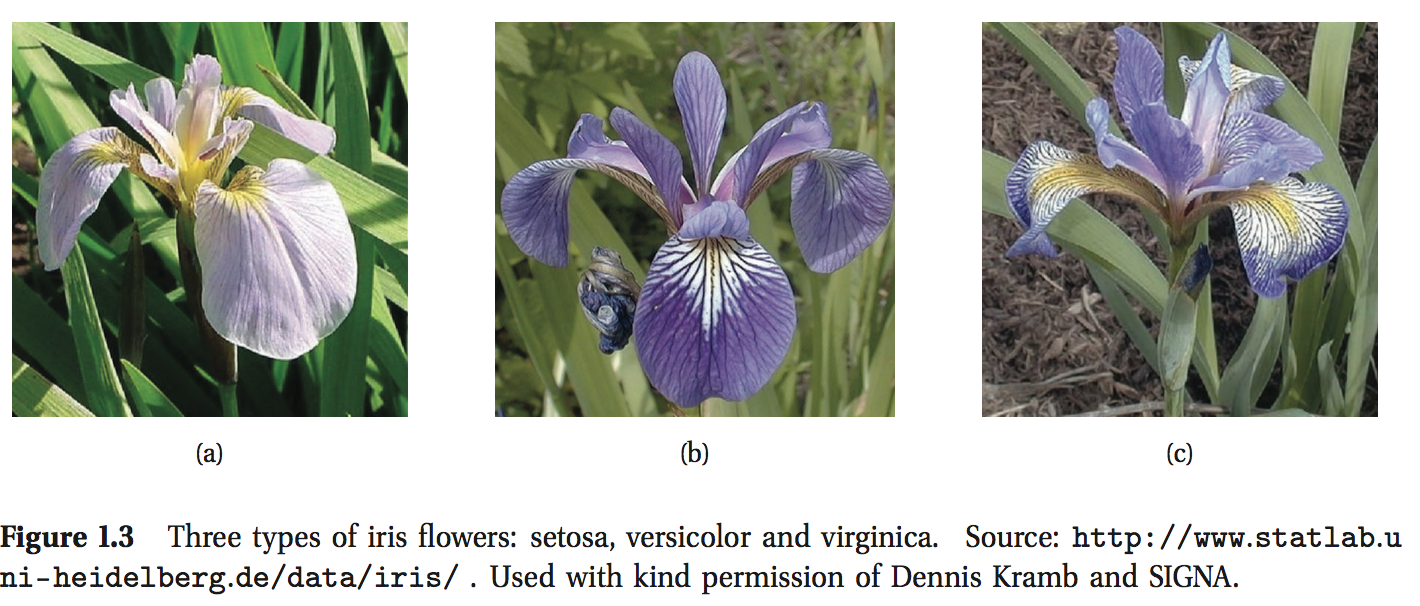
\includegraphics[width=9\textwidth]{figs/flores}
  \end{textblock}


  \begin{textblock}{5}(9.5,13.5)
  ¿Cómo elegir las características?
\end{textblock}


  }
  \frame[t]{\frametitle{Aprendizaje supervisado (Regresión)}
Similar a clasificación, pero el espacio de llegada es continuo.\\
- En general, elegimos una función $x\rightarrow y=f(x,\theta)$ y encontramos $\theta$ de acuerdo a una figura de mérito\\
- ¿qué estructura tiene $f(\cdot,\theta)$?\\
- Ejemplos: predicción financiera, sondaje, control predictivo, reconstrucción y filtrado:

\begin{textblock}{1}(1,7.5)
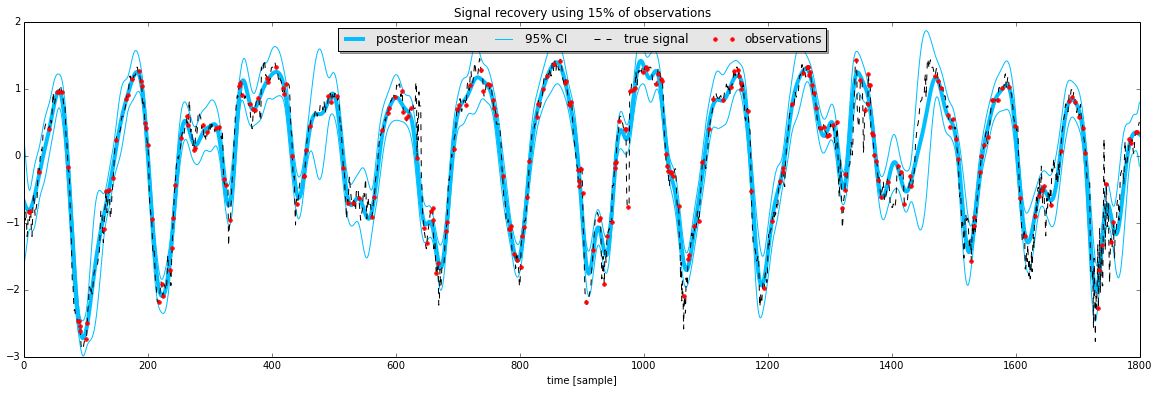
\includegraphics[width=14\textwidth]{figs/heart_rate}\\
\end{textblock}
\begin{textblock}{13}(1,14)
\small{\red{figura:} reconstrucción de una señal de frecuencia cardíaca en base al 20\% de las mediciones usando procesos Gaussianos}
\end{textblock}


  }




  \frame[t]{\frametitle{Aprendizaje no supervisado}
  Etiquetas no disponibles: el objetivo es descubrir estructura en los datos.\\
  El producir datos etiquetados (por humanos) no es solo costoso sino que contiene información parcial; por el contrario, al considerar directamente los datos mucha más información puede ser extraída.\\
  Ejemplos:\\
  - cluster\\
  - density estimation\\
  - PCA\\
  - Image impainting \\
  - Filtrado colaborativo (Netflix)

  \begin{textblock}{1}(9,11)
  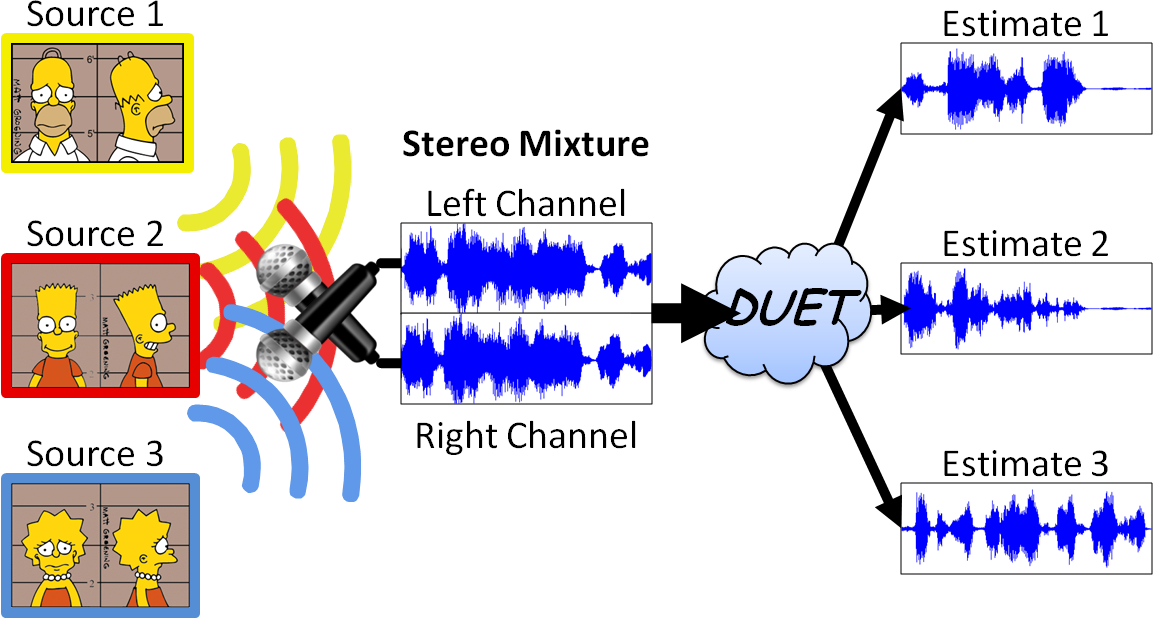
\includegraphics[width=6\textwidth]{figs/ss}\\
  \end{textblock}

  \begin{textblock}{1}(1,11)
  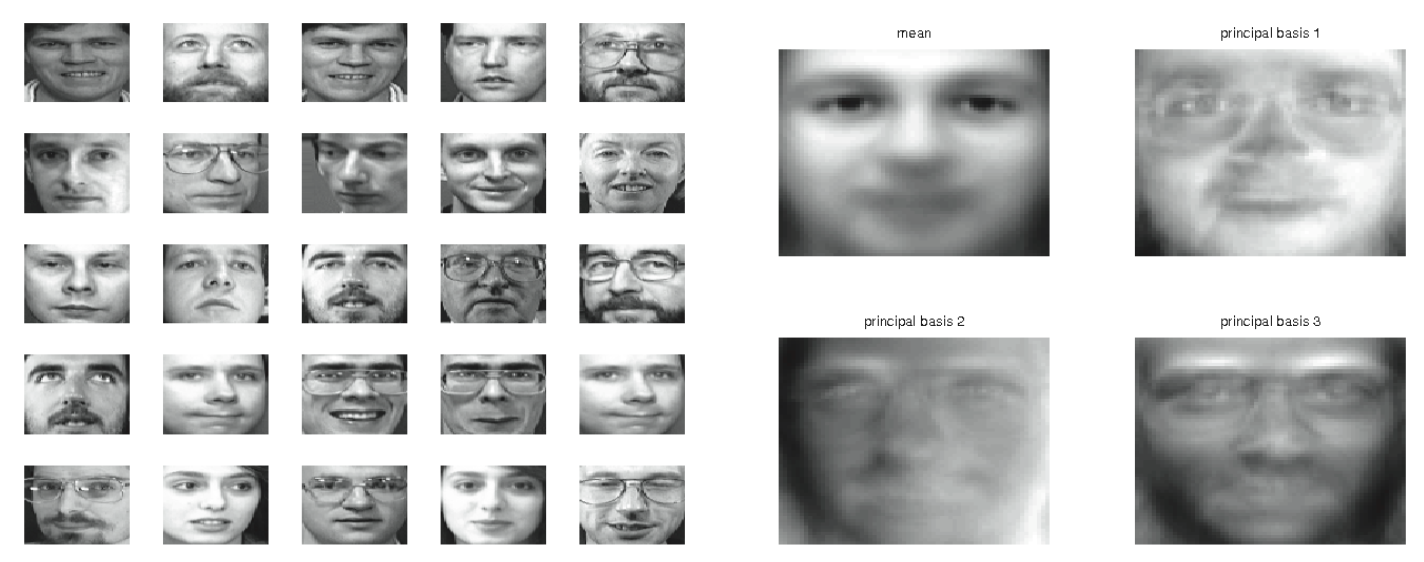
\includegraphics[width=7\textwidth]{figs/faces}\\
  \end{textblock}

  \begin{textblock}{1}(9,6.5)
  
\includegraphics[width=4\textwidth]{figs/netflix}\\
  \end{textblock}

   }



   \frame[t]{\frametitle{Aprendizaje reforzado}
 Aprender a tomar decisiones en base a una señal de recompenza o penalización.\\
 \vspace{3cm}
 - Aprendizaje en humanos y animales sigue este concepto\\
 - Aplicaciones en robótica, juegos de video, finanzas, etc
 \begin{textblock}{1}(4,3.5)
 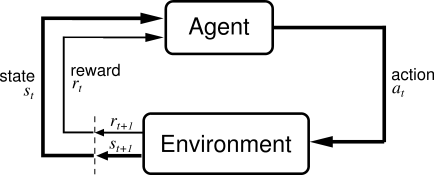
\includegraphics[width=8\textwidth]{figs/rl}\\
 \end{textblock}

 \begin{textblock}{1}(1,11)
 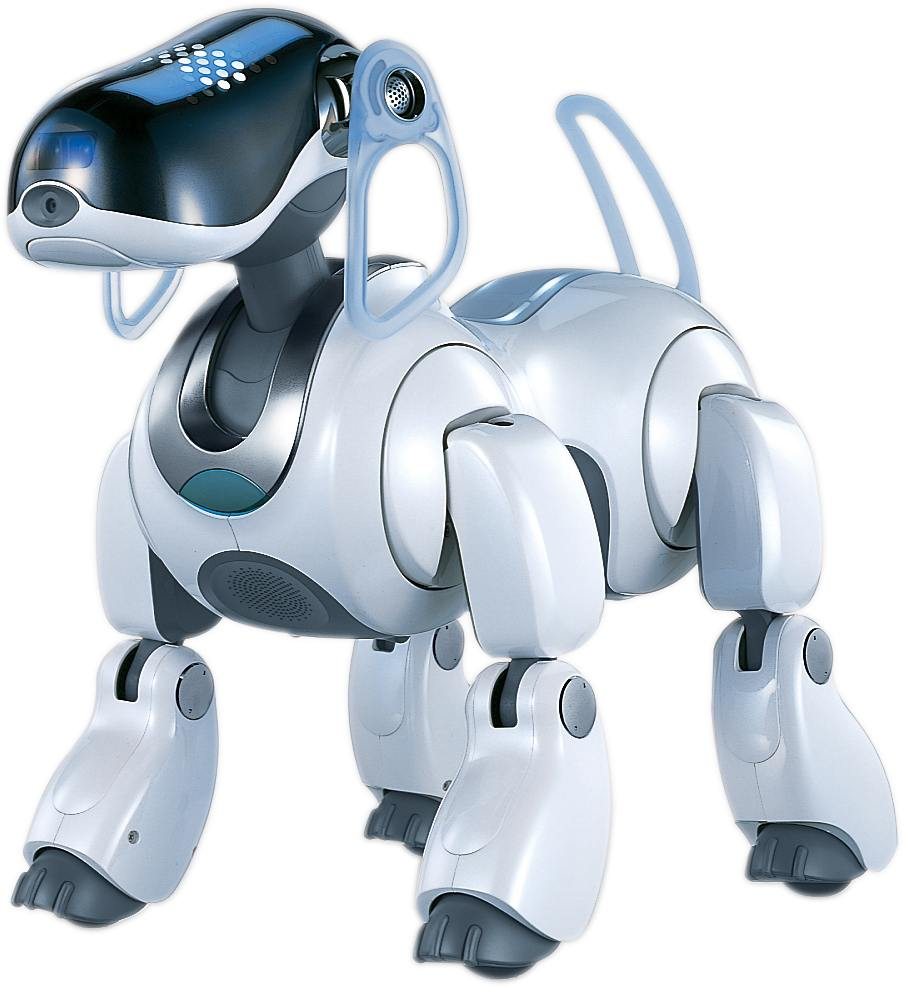
\includegraphics[width=3\textwidth]{figs/aibo}\\
 \end{textblock}

 \begin{textblock}{1}(5,11)
 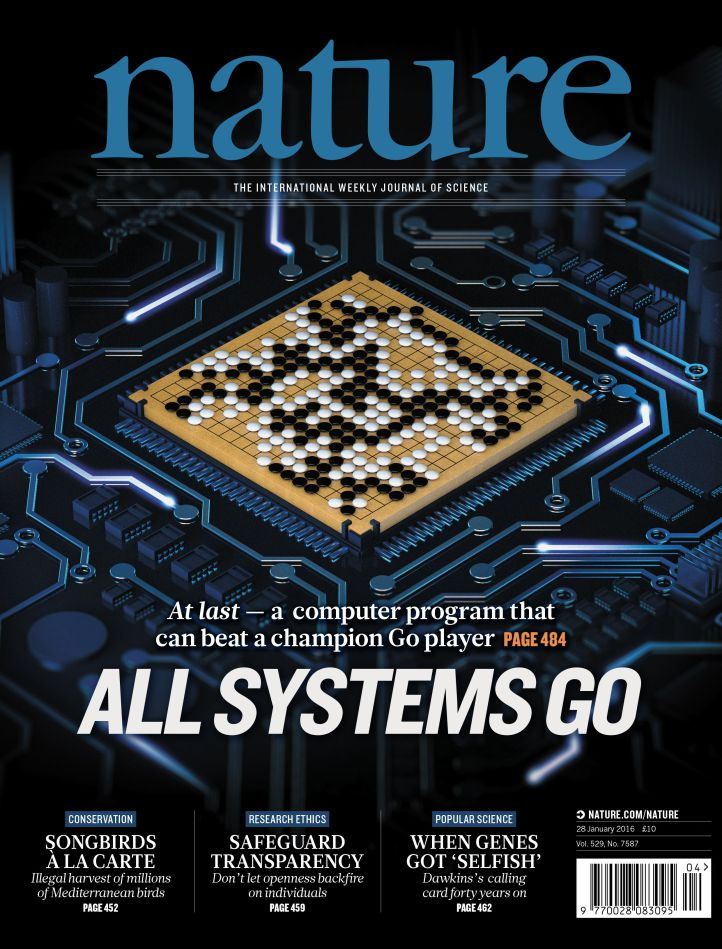
\includegraphics[width=2.5\textwidth]{figs/nature}\\
 \end{textblock}


 \begin{textblock}{1}(9,11)
 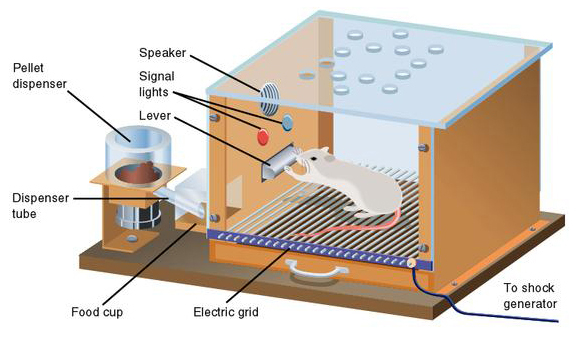
\includegraphics[width=5\textwidth]{figs/skinner}\\
 \end{textblock}




    }

  

    \frame{\frametitle{Aprendizaje de máquinas: ¿Qué hacer?}
\vspace{-2cm}
\begin{itemize}
  \item  MA5204: lunes y miércoles a las 830am
    \item Unirse  a GAMES: \url{games.cmm.uchile.cl}
    \item Aprender algún lenguaje de programación (e.g., Python)
    \item MOOCs: Coursera, MIT OCW, \textit{Learning from data} (Stanford)
    \item podcasts: \url{http://www.thetalkingmachines.com/}
    \item libros
\end{itemize}


    \begin{textblock}{30}(1.5,9.5)
      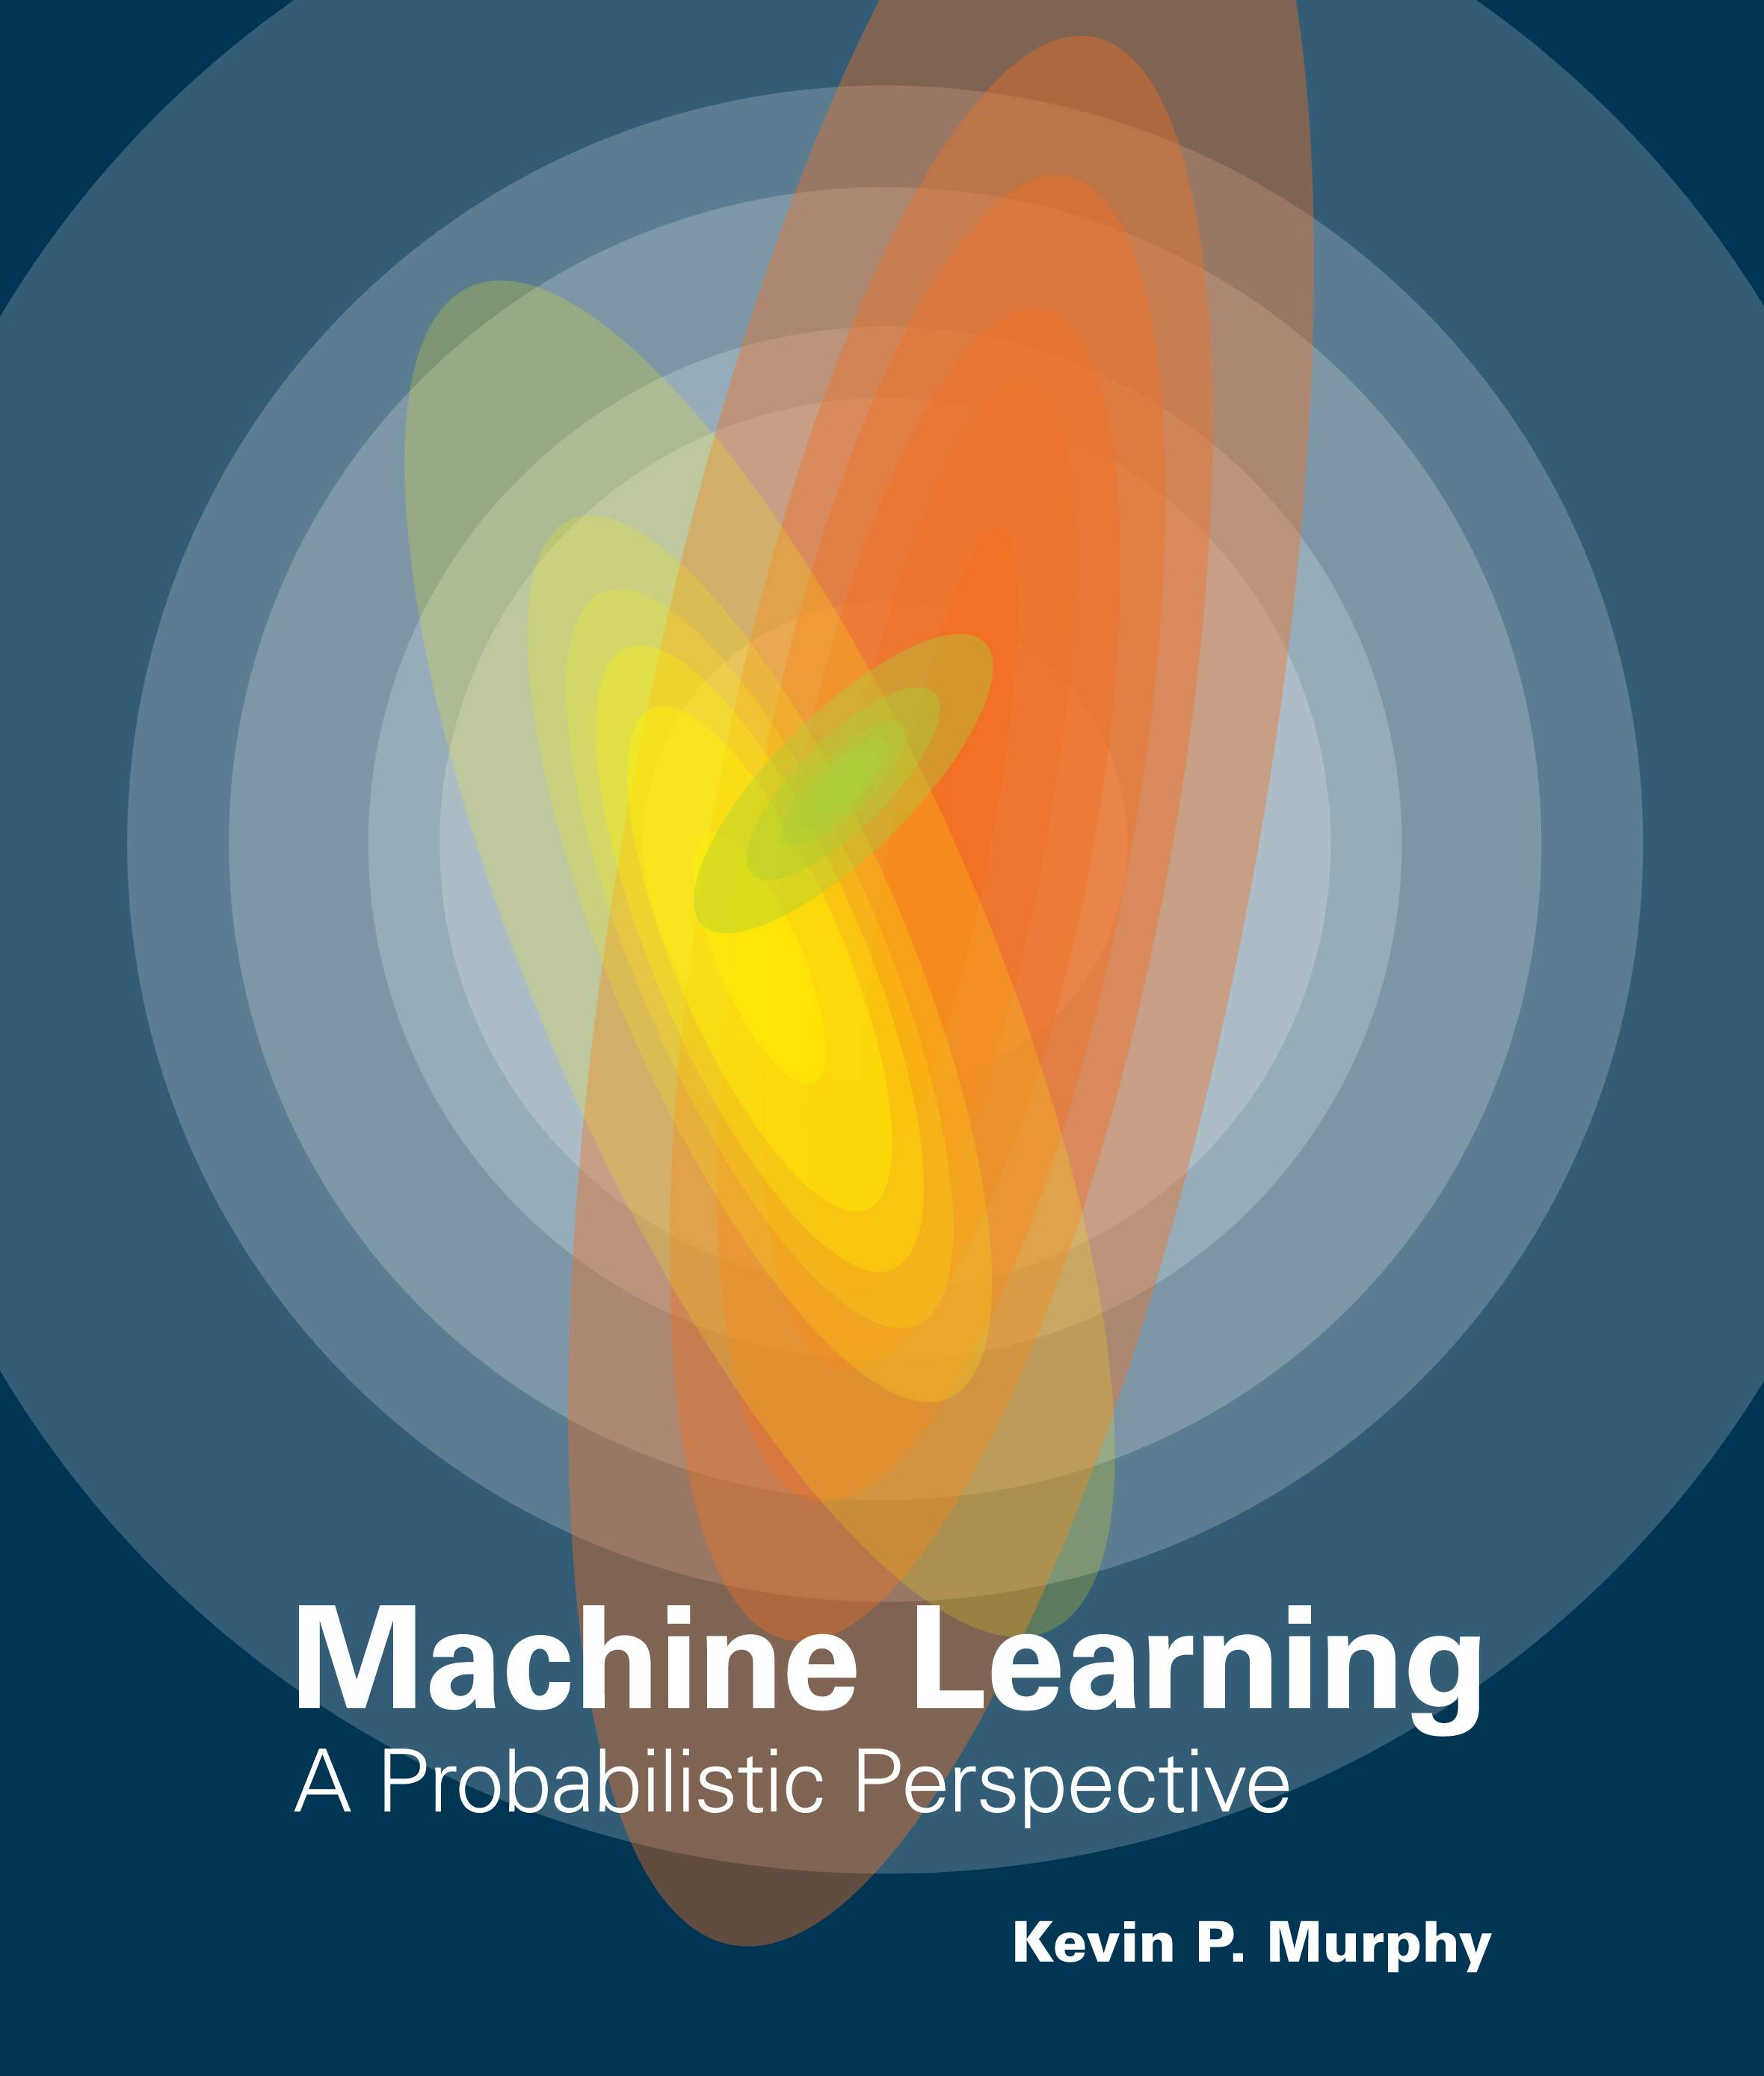
\includegraphics[width=.1\textwidth]{figs/murphy} \quad 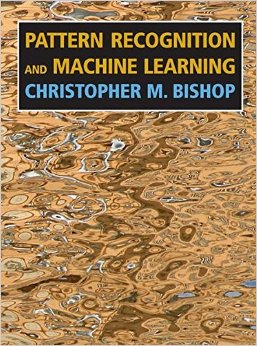
\includegraphics[width=.1\textwidth]{figs/bishop} \quad
        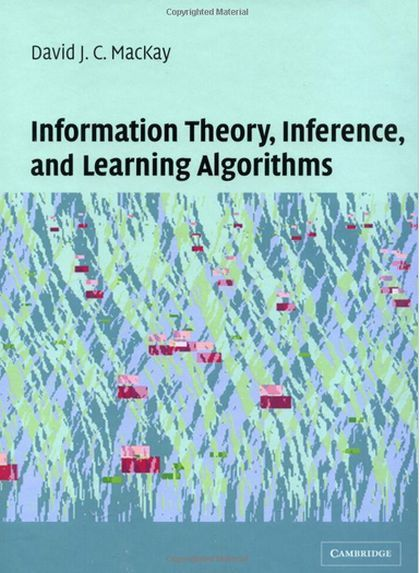
\includegraphics[width=.1\textwidth]{figs/mackay} \quad
          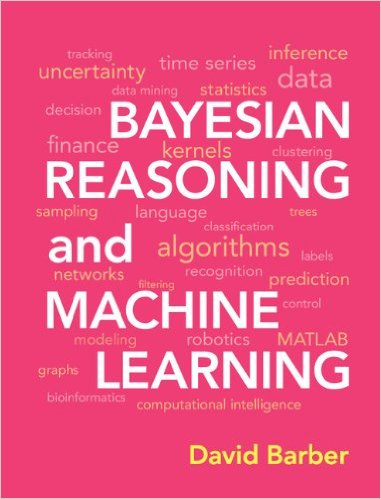
\includegraphics[width=.1\textwidth]{figs/barber}
    \end{textblock}






    }


\end{document}
